\documentclass[12pt]{report}
\usepackage[print,nopanel]{pdfscreen}
\begin{print}
\usepackage{lipsum}
\usepackage{titletoc}
\usepackage{lastpage}
\usepackage{macro/macro}
\usepackage{float}
\usepackage{wrapfig}
\usepackage{fancyhdr}
\usepackage{verbatim}
\usepackage{scrextend}
\usepackage{array}


\usepackage[Glenn]{fncychap}
\lhead{\large\bfseries\   }
\usepackage[left=3.5cm, right=1.25cm, top=2.5cm, bottom=1.25cm]{geometry}
\pagestyle{fancy}
\end{print}
\margins{.5cm}{.5cm}{.5cm}{.5cm}
\begin{screen}

\renewcommand{\encodingdefault}{T1}
\usepackage{setspace}
\linespread{1.5}
\renewcommand{\rmdefault}{ptm}
\end{screen}
\screensize{8cm}{9cm}
\overlay{overlay8.pdf}
\usepackage{graphicx}

\usepackage{listings}

\newcommand{\studentName}{Gursimar Singh}
\newcommand{\studentRollNo}{1411256}
\newcommand{\appName}{Retinal Image Enhancement}

\makeatletter
\def\@makechapterhead#1{%
	%%%%\vspace*{50\p@}% %%% removed!
	{\parindent \z@ \raggedright \normalfont
		\ifnum \c@secnumdepth >\m@ne
		\huge\bfseries 	\@chapapp\space \thechapter
		\par\nobreak
		\vskip 20\p@
		\fi
		\interlinepenalty\@M
		\Huge \bfseries #1\par\nobreak
		\vskip 40\p@
}}
\def\@makeschapterhead#1{%
	%%%%%\vspace*{50\p@}% %%% removed!
	{\parindent \z@ \raggedright
		\normalfont
		\interlinepenalty\@M
		\Huge \bfseries  #1\par\nobreak
		\vskip 40\p@
}}
\makeatother

\begin{document}
\newcommand{\centertext}[1]{\begin{center}\textbf{#1}\end{center}}
\newcommand{\student}{\vskip 2.5cm}
\newcommand{\supervisor}{\vskip 2cm}
\newcommand{\stamp}{\vskip 2.5cm}
\newcommand{\HRule}{\rule{\linewidth}{0.5mm}}
\newcommand{\projecttitle}{\Huge {Retinal Image Enhancement  }\vskip 0.1in}
\newcommand{\tab}[1]{\hspace{.4\textwidth}\rlap{#1}}
\newcommand{\itab}[1]{\hspace{.05\textwidth}\rlap{#1}}
\newcommand{\logo}[1]{\includegraphics[scale=0.7]{#1}}
\newcommand{\submitted}{


\vskip 0.2in
\vskip 0.7cm
\large\bf{\bf REPORT}\\
\vskip 0.5cm
\textnormal{
SUBMITTED IN PARTIAL FULFILLMENT OF THE REQUIREMENT FOR
THE AWARD OF THE DEGREE OF 
}
\vskip 0.2cm

\vskip 0.2cm

\large\bf{\bf BACHELOR OF TECHNOLOGY}\\
\textnormal{(INFORMATION TECHNOLOGY)}


\vskip 1.7cm
\textnormal{Submitted By \vspace{5pt} \\
	\studentName \ (\studentRollNo)\\
      Kuvarpreet Singh (1411276) \\ Gursimran Singh Basra (1411258) 
 }

\vskip 0.5cm
%\image{0.7}{images/gne.png}{}
\logo{images/gne.png}
\vskip 3.0cm


%\image{0.7}{images/gne.png}{}
%\logo{images/gne.png}
%\vskip 3.0cm

\HRule \\[0.4cm]

\textnormal \bf{ \bf Information Technology Department} 
\large \bf{ \bf \\GURU NANAK DEV ENGINEERING COLLEGE } 
\large { \\LUDHIANA, INDIA }
 }


\newcommand{\pagetitle}{\begin{center}
\projecttitle
\Large\textbf{}\\
\submitted
\vskip 1cm

\end{center}}
\newcommand{\openoffice}{\textbf{OpenOffice}}
\newcommand{\frontmatter}[1]{\begin{Large} \textbf{#1} \end{Large}}
\newcommand{\ppttitle}{\begin{center}
\end{center}}

\begin{screen}
\ppttitle
\end{screen}
\footskip 0.7cm
\thispagestyle{empty} 
\pagetitle

\pagenumbering{Roman}
\newpage
%\cfoot{\thepage}
%\begin{Large}
\centertext{Certificate}
\end{Large}
\vskip 0.1in \noindent I hereby certify that the work which is being submitted in this project titled \textbf{"Automated Buiding Drawings"},
in partial fulfilment of the requirement for the award of degree of Bachelors of Technology in Computer
Science and Engineering submitted in Guru Nanak Dev Engineering College, Ludhiana, is an authentic
record of my own work carried out under the supervision of Mrs. Sumeet Kaur Sehra.\\\\\vskip 0.3in
\noindent\textbf{(Mandeep Singh)}\\
Roll No.: 125045 \\
University Registration No.: 1243667 \\\\\vskip 0.3in

\noindent\textbf{(Navdeep Singh)}\\
Roll No.: 125051 \\
University Registration No.: 1243678 \\\\\vskip 0.2in

\noindent This is to certify that the statements made above by the candidate are correct and true to the best of my knowledge.\\\\\\\\


\noindent \textbf{(Mrs. Sumeet Kaur Sehra)}\\
Assistant Professor\\
Computer Science and Engineering Department\\
Guru Nanak Dev Engineering College\\
Ludhiana-141006
\begin{Large}
\centertext{Abstract}
\end{Large}
\vskip 0.1in Retinal Images are very important for the identification of various eye related diseases and various more issues related to body. \\  

\noindent The web application technologies is one of the top-selling in the world, it is apparent that people have been using systems as an organizational tool.\\

\noindent Retinal Image Enhancement is the web application made for medical staff who work on retinal images to provide a better judgement on the retinal images.This web application contains various options of image enhancement techniques in which the best one could be selected..Through our application medical staff can
easily easily find the best image and be able to provide proper assesment of vaious eye related issues.
\newpage
\label{•} \begin{Large}
\centertext{Acknowledgement}
\end{Large}
\vskip 0.1in % "I am  highly grateful to ​
%Dr. M.S. Saini Director, Guru Nanak Dev Engineering  
%College, Ludhiana for providing this opportunity to carry out minor project at Guru Nanak  
%Dev Engineering College. The constant guidance and encouragement received from ​
%ER. Inderjeet Singh, Assistant Professor, Department of IT has been of great help in carrying out the project work and is acknowledged with reverential thanks.

%I would like to express a deep sense of gratitude and thanks profusely to DR. K.S. Mann, Guru Nanak Dev Engineering College. Without his wise counsel and able guidance, it would have been impossible to complete the report in this manner. The author expresses gratitude to other faculty members of IT department of GNDEC for their intellectual support throughout the course of this work.

%Last, but not the least I wish to thank my parents and friends who directly or indirectly have given me moral support and their relentless advice throughout the completion of this project work.% 

\noindent We are highly grateful to the Dr. SEHIJPAL SINGH KHANGURA, Guru Nanak Dev Engineering College (GNDEC), Ludhiana, for providing this opportunity to carry out the major project work at Guru Nanak Dev Engineering College.\\

\noindent The constant guidance and encouragement received from Dr.Amit Kamra from IT Department, GNDEC Ludhiana has been of great help in carrying out the project work and is acknowledged with reverential thanks.\\

\noindent We would like to express a deep sense of gratitude and thanks profusely to Dr Amit kamra, without his wise counsel and able guidance, it would have been impossible to complete the project in this manner.\\

\noindent We express gratitude to other faculty members of Information Technology department of GNDEC for their intellectual support throughout the course of this work.\\

\noindent Finally, we are indebted to all whosoever have contributed in this report work.



\vskip 0.4in
\noindent 
\textbf{Gursimar Singh}\\
\textbf{Gursimran Singh Basra}\\
\textbf{Kuvarpreet Singh}
%\textbf {Navjot Singh}\\ \noindent \textbf{Manpreet Singh}\\ \noindent \textbf{Deepak Pruthi}


\newpage
\listoffigures
\newpage

\listoftables

\newpage
\tableofcontents
\newpage


\pagenumbering{arabic}
\cfoot{\thepage}

\newpage
\chapter{Introduction}
\section{Introduction To Project} 
Retinal fundus images provide rich information of pathological changes which may indicate
diseases such as arteriosclerosis, diabetes, hypertension, stroke, and cardiovascular disease.
the project will help doctors and medical technicians to get better assessment of the image
and so that they can help the patient with their diagnosis. We used DRIVE database for the
sample retinal imagesand we will apply various enhancement techniques and provide qualitative
analysis of given images.

\section{Project Category(Internet based, Application or System Development)}
This application is research based application .

\section{Objectives}

\begin{itemize}
	\item  To study the enhancement of retinal image.

	\item To process an retinal image so that the output image is more enhanced than the original image..
	
	\item To perform the objective evaluation of the result and tell about the best image.


\end{itemize}

\section{Problem Formulation}
Through our project, medical team or doctors will be able to give a better assessment of the images for the proper treatment of the various eye related problems and can help in find out about various eye realted diseases  .   

\section{Proposed System Modules}

\begin{itemize}
	\item User will be able to select retinal image for various image operations.

	\item Time will be saved as doctors will find the disease much faster through the image  .
	
	\item Medical team will give assesment about the best possible image.   
	
	
	


\end{itemize}

 
\section{Unique Features of the System}
\begin{itemize}

\item Time will be saved as doctors will find the disease much faster through the image  .
\item To process an retinal image so that the output image is more enhanced than the original image.

\item User will be able to select retinal image for various image operations..

\item Medical team will give assesment about the best possible image.

\end{itemize}



\newpage
%\chapter{\LaTeX}
%

\LaTeX, I have used this tool for preparing my six weeks training report and i found it excellent. So this time again i decided to use it for my report.
\LaTeX{} (pronounced /ˈleɪtɛk/, /ˈleɪtɛx/, /ˈlɑːtɛx/, or /ˈlɑːtɛk/) is a 
document markup language and document preparation system for the \TeX{} 
typesetting  program. Within the typesetting system, its name is styled 
as \LaTeX.

\image{0.9}{images/donald.png}{Donald Knuth, Inventor Of \TeX{} 
typesetting system}

\noindent Within the typesetting system, its name is styled as \LaTeX. The term 
\LaTeX{} refers only to the language in which documents are written, 
not to the editor used to write those documents. In order to create a 
document in \LaTeX, a .tex file must be created using some form of text 
editor. While most text editors can be used to create a \LaTeX{} document, 
a number of editors have been created specifically for working with \LaTeX.\\

\noindent \LaTeX{} is most widely used by mathematicians, scientists, 
engineers, philosophers, linguists, economists and other scholars in 
academia. As a primary or intermediate format, e.g., translating DocBook 
and other XML-based formats to PDF, \LaTeX{} is used because of the 
high quality of typesetting achievable by \TeX. The typesetting system 
offers programmable desktop publishing features and extensive facilities 
for automating most aspects of typesetting and desktop publishing, 
including numbering and cross-referencing, tables and figures, 
page layout and bibliographies.\\

\noindent \LaTeX{} is intended to provide a high-level language that
accesses the power of \TeX. \LaTeX{} essentially comprises a
collection of \TeX{} macros and a program to process \LaTeX documents. 
Because the \TeX{} formatting commands are very low-level, it is usually 
much simpler for end-users to use \LaTeX{}.


\section{Typesetting}
\LaTeX{} is based on the idea that authors should be able to focus on 
the content of what they are writing without being distracted by its 
visual presentation. In preparing a \LaTeX{} document, the author 
specifies the logical structure using familiar concepts such as 
chapter, section, table, figure, etc., and lets the \LaTeX{} system 
worry about the presentation of these structures. It therefore 
encourages the separation of layout from content while still allowing 
manual typesetting adjustments where needed. 

\begin{verbatim}
\documentclass[12pt]{article}
\usepackage{amsmath}
\title{\LaTeX}
\date{}
\begin{document}
  \maketitle 
  \LaTeX{} is a document preparation system 
  for the \TeX{} typesetting program.
   \par 
   $E=mc^2$
\end{document}
\end{verbatim}

\subsection{Installing \LaTeX{} on System}
Installation of \LaTeX{} on personal system is quite easy. As i have used \LaTeX{} on Ubuntu 14.04 so i am discussing the installation steps for Ubuntu 14.04 here:\\
\begin{itemize}
\item Go to terminal and type\\
\textit{sudo apt-get install texlive-full}
\item Your Latex will be installed on your system and you can check for manual page by typing.\\
\textit{man latex}
in terminal which gives manual for latex command.
\item To do very next step now one should stick this to mind that the document which one is going to produce is written in any type of editor whether it may be your most common usable editor Gedit or you can use vim by installing first vim into your system using command.\\
\textit{sudo apt-get install vim}
\item After you have written your document it is to be embedded with some set of commands that Latex uses so as to give a structure to your document. Note that whenever you wish your document to be looked into some other style just change these set of commands.
\item When you have done all these things save your piece of code with .tex format say test.tex. Go to terminal and type\\
\textit{latex path of the file test.tex Or pdflatex path of the file test.tex\\ eg: pdflatex test.tex}
for producing pdf file simultaneously.\\
After compiling it type command\\\\
\textit{evince filename.pdf\\ eg: evince test.pdf}\\
To see output pdf file. 
\end{itemize}

\subsection{Graphical Editors for \LaTeX{}}
\LaTeX{} is not restricted to command line only there are so many graphical based editors available to be used. These GUi based editors provide an easy interface to user so as to do typesetting in an efficient manner. Some of them are listed below:
\begin{itemize}
\item Tex Maker
\item LED 
\end{itemize}
And many more but the preferred method to produce \LaTeX{} document is through console mode only.

%\chapter{Literature Review}
%

\chapter{Requirement Analysis and System Specification}
\section{Feasibility Study (Technical,Economical,Operational)}
Feasibility study is made to see if the project on completion will serve the purpose of the organization for the amount of work, effort and the time that spend on it. Feasibility study lets the developer foresee the future of the project and the usefulness. A feasibility study of a system proposal is according to its workability, which is the impact on the organization, ability to meet their user needs and effective use of resources. Carrying out a feasibility study involves information assessment, information collection and report writing. The information assessment phase identifies the information that is required to answer the three questions set out above. Once the information has been identified, you should question information sources to discover the answers to these questions Thus when a new application is proposed it normally goes through a feasibility study before it is approved for development.

A feasibility study is designed to provide an overview of the primary issues related to a business idea.  The purpose is to identify any “make or break” issues that would prevent your business from being successful in the marketplace. In other words, a feasibility study determines whether the business idea makes sense. A thorough feasibility analysis provides a lot of information necessary for the business plan.  For example, a good market analysis is necessary in order to determine the project’s feasibility.  This information provides the basis for the market section of the business plan.

The document provide the feasibility of the project that is being designed and lists various areas that were considered very carefully during the feasibility study of this project such as Technical, Economic and Operational feasibilities. Feasibility is defined as the practical extent to which a project can be performed successfully. To evaluate feasibility, a feasibility study is performed, which determines whether the solution considered to accomplish the requirements is practical and workable in the software. Information such as resource availability, cost estimation for software development, benefits of the software to the organization after it is developed and cost to be incurred on its maintenance are considered during the feasibility study. The objective of the feasibility study is to establish the reasons for developing the software that is acceptable to users, adaptable to change and conformable to established standards.

Objectives of feasibility study are listed below.
\begin{itemize}
	\item To analyze whether the software will meet organizational requirements
	\item To determine whether the software can be implemented using the current technology and within the specified budget and schedule
	\item To determine whether the software can be integrated with other existing software.
\end{itemize}

\subsection{Types of Feasibility}
Various types of feasibility that are commonly considered include technical feasibility, operational feasibility, and economic feasibility.

\subsubsection{Technical Feasibility}
Technical feasibility is one of the first studies that must be conducted after the project has been identified. In large engineering projects consulting agencies that have large
staffs of engineers and technicians conduct technical studies dealing with the projects. 

When writing a feasibility report, the following should be taken to consideration:
\begin{itemize}
	\item A brief description of the business to assess more possible factors which could affect the study
	\item The part of the business being examined
	\item The human and economic factor
	\item The possible solutions to the problem
\end{itemize}

The system must be evaluated from the technical point of view first. The assessment of this feasibility must be based on an outline design of the system requirement in the terms of input, output, programs and procedures. Having identified an outline system, the investigation must go on to suggest the type of equipment, required method developing the system, of running the system once it has been designed. Technical feasibility assesses the current resources (such as hardware and software) and technology, which are required to accomplish user requirements in the software within the allocated time and budget. For this, the software development team ascertains whether the current resources and technology can be upgraded or added in the software to accomplish specified user requirements. Technical feasibility also performs the following tasks.

\begin{itemize}
	\item Analyzes the technical skills and capabilities of the software development team members
	\item Determines whether the relevant technology is stable and established
	\item Ascertains that the technology chosen for software development has a large number of users so that they can be consulted when problems arise or improvements are required.
\end{itemize}

Technical issues raised during the investigation are:
\begin{itemize}
	\item Does the existing technology sufficient for the suggested one?
	\item Can the system expand if developed?
\end{itemize}

The project should be developed such that the necessary functions and performance are achieved within the constraints. The project is developed within latest technology. Through the technology may become obsolete after some period of time, due to the fact that never version of same software supports older versions, the system may still be used. So there are minimal constraints involved with this project. The system has been developed using Java the project is technically feasible for development.

\subsubsection{Economic Feasibility}
The purpose of the economic feasibility assessment is to determine the positive economic benefits to the organization that the proposed system will provide. It includes quantification and identification of all the benefits expected. This assessment typically involves a cost/ benefits analysis.

Software is said to be economically feasible if it focuses on the issues listed below.
\begin{itemize}
	\item Cost incurred on software development to produce long-term gains for an organization.
	\item Cost required to conduct full software investigation (such as requirements elicitation and requirements analysis).
	\item Cost of hardware, software, development team, and training.
\end{itemize}

The following are some of the important financial questions asked during preliminary investigation:
\begin{itemize}
	\item The costs conduct a full system investigation.
	\item The cost of the hardware and software.
	\item The benefits in the form of reduced costs or fewer costly errors.
\end{itemize}

Since the system is developed as part of project work, there is no manual cost to spend for the proposed system. Also all the resources are already available, it give an indication of the system is economically possible for development.

\subsubsection{Operational Feasibility}
If the system is not easy to operate, than operational process would be difficult. The operator of the system should be given proper training. The system should be made such that the user can interface the system without any problem.

Operational feasibility is a measure of how well a proposed system solves the problems, and takes advantage of the opportunities identified during scope definition and how it satisfies the requirements identified in the requirements analysis phase of system development. The operational feasibility assessment focuses on the degree to which the proposed development projects fits in with the existing business environment and objectives with regard to development schedule, delivery date, corporate culture, and existing business processes.

Operational feasibility also performs the following tasks.

\begin{itemize}
	\item Determines whether the problems anticipated in user requirements are of high priority.
	\item Determines whether the solution suggested by the software development team is acceptable.
	\item Analyzes whether users will adapt to a new software.
	\item Determines whether the organization is satisfied by the alternative solutions proposed by the software development team.
\end{itemize}

This includes the following questions:
\begin{itemize}
	\item Is there sufficient support for the users?
	\item Will the proposed system cause harm?
	\item The project would be beneficial because it satisfies the objectives when developed and installed. All behavioral aspects are considered carefully and conclude that the project is behaviorally feasible.
\end{itemize}

This system proposed will have a very user friendly interface, a naïve user will be able to understand the user interface in seconds. It’ll have basic yet intriguing interface with a feature of adding news and pictures,bottom slider which will operate the admin to add news and many other functions which is easily understandable.

\section{Software Requirement Specification Document}
\subsection{Data Requirement}
For this project, we used retinal images for testing available at DRIVE database. Also we have gathered information from research paper written by Nidhi Singla and Navdeep Singh (2017), Rajesh Garg et al. (2011), Parul and Neetu Sharma (2015), Agung W. Setiawan, et al. (2013).    

\subsection{Performance Requirement}
Basis on resource requirements, this application will be able to run on pretty low-end devices with 512MB of ram and 800Mhz processor.

\subsection{Functional Requirement}
This application will take retinal image input from the user and then will perform various operations to detect various abnormalities in retina.    

\section{Intended User}
Medical staff responsible for assesment of retinal images will use our project. To provide the better assesment of the retinal image, our project will come in use.  

\section{Features}
\begin{itemize}
	\item User will be able to add retinal images for the assesment.
	
	\item Time consuming will be less due to early assesment of the retinal images.
	 
\end{itemize}

	 	
\section{Expected hurdles}
\begin{itemize}
\item Browsing the retinal images.  
\item Gathering various information about retina from different research image.
\item Dependencies of the different libraries used in the project.

\end{itemize}

\section{SDLC model to be used}
\subsection{Agile Model}

 Agile modeling (AM) is a methodology for modeling and documenting software systems based on best practices. It is a collection of values and principles, that can be applied on an (agile) software development project. This methodology is more flexible than traditional modeling methods, making it a better fit in a fast changing environment.[1] It is part of the agile software development tool kit.
 
Agile development model is also a type of Incremental model. Software is developed in incremental, rapid cycles. This results in small incremental releases with each release building on previous functionality. Each release is thoroughly tested to ensure software quality is maintained. It is used for time critical applications.  Extreme Programming (XP) is currently one of the most well known agile development life cycle model. 
\begin{figure}[ht]
\centering
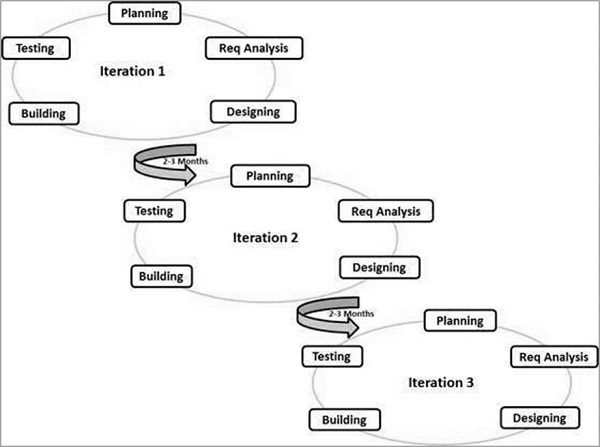
\includegraphics[scale=0.5]{images/AgileModel.jpg}
\caption{Agile Model}
\end{figure}


%\newpage

%\chapter{Technologies Used}
%
\section{Introduction to PHP}
\begin{figure}[h]
\centering \includegraphics[scale=0.4]{images/php.png}
\caption{Php logo}
\end{figure}
\noindent PHP is an open source server-side scripting language designed for Web development to produce dynamic Web pages. It is one of the first developed server-side scripting languages to be embedded into an HTML source document rather than calling an external file to process data. The code is interpreted by a Web server with a PHP processor module which generates the resulting Web page. It also has evolved to include a command-line interface capability and can be used in standalone graphical applications.\\

\noindent PHP can be deployed on most Web servers and also as a standalone shell on almost every operating system and platform, free of charge. A competitor to Microsoft’s Active Server Pages (ASP) server-side script engine and similar languages, PHP is installed on more than 20 million Web sites and 1 million Web servers. Notable software that uses PHP includes Drupal, Joomla, MediaWiki, and WordPress. PHP is a general-purpose scripting language.\\

\noindent It is especially suited to server-side web development where PHP generally runs on a web server. Any PHP code in a requested file is executed by the PHP runtime, usually to create dynamic web page content or dynamic images used on Web sites or elsewhere. It can also be used for command-line scripting and client-side graphical user interface (GUI) applications. PHP can be deployed on most Web servers, many operating systems.
\subsection{Features of PHP}
\begin{itemize}
\item Http Authentication
\item Cookies and Sessions
\item Connection Handling
\item Designer-friendly 
\item Cross platform Compatibility 
\item Loosely typed Language
\item Open Source
\item Easy code
\end{itemize}



\section{MySQL Database Server}
\begin{figure}[h]
\centering \includegraphics[scale=0.2]{images/mysql.jpg}
\caption{Mysql logo}
\end{figure}
\noindent I used the Mysql database for my project. It is world''s most popular open source database It 
is a relational database management system (RDBMS) that runs as a server 
providing multi-user access to a number of databases. It is named after 
developer Michael Widenius's daughter, My. The SQL phrase stands for
Structured Query Language. MySQL is written in C and C++.\\

\noindent Free-software-open source projects that require a 
full-featured database management system
often use MySQL. MySQL is also used in many high-profile, large-scale World 
Wide Web products, including
Wikipedia, Google (though not for searches) and Facebook.\\

\noindent MySQL is a popular choice of database for use in web 
applications, and is a central component of the widely used LAMP web 
application software LAMP is an acronym for “Linux, Apache, MySQL, 
Perl/PHP/Python”. MySQL is used in some of the most frequently visited web sites 
on the Internet, including Flickr, Nokia.com, YouTube, Wikipedia, Google 
and Facebook.\\

\noindent One of the greatest advantage of Django is that it synchronises the 
database only with one command withouut having any need to send 
different queries for insertion, deletion, updation etc. There is a 
file named models.py which is used for purpose of creating database.
\subsection{Features of MySQL}
\begin{itemize}
\item MySQL is a database management system.
\item MySQL is a relational database management system.
\item MySQL software is Open Source.
\item The MySQL Database Server is very fast, reliable, and easy to 
use.
\item MySQL Server works in client/server or embedded systems.
\item A large amount of contributed MySQL software is available.
\end{itemize}
\subsection{Installation of MySQL}
MySql can be installed using following commands:\\

\hspace{4pt} \$ sudo apt-get install mysql-server\\

\hspace{4pt} \$ sudo apt-get install mysql-client


\section{Introduction to Bootstrap} 

\begin{figure}[h]
\centering \includegraphics[scale=0.3]{images/bootstrap.png}
\caption{Bootstrap logo}
\end{figure}
\subsection{What is Bootstrap}
\noindent Bootstrap is a powerful front-end framework for faster and easier web development. It includes HTML and CSS based design templates for common user interface components like Typography, Forms, Buttons, Tables, Navigations, Dropdowns, Alerts, Modals, Tabs, Accordion, Carousel and many other as well as optional JavaScript extensions.
Bootstrap also gives you ability to create responsive layout with much less efforts.
\subsection{Advantages of Bootstrap}
The biggest advantage of using Bootstrap is that it comes with free set of tools for creating flexible and responsive web layouts as well as common interface components.
Additionally, using the Bootstrap data APIs you can create advanced interface components like Scrollspy and Typeaheads without writing a single line of JavaScript.
Here are some more advantages, why one should opt for Bootstrap:
\begin{itemize}
\item Save lots of time.
\item Responsive features.
\item Consistent design .
\item Easy to use.
\item Compatible with browsers.
\item Open Source.
\item Consistency.
\item Comprehensive List Of Components
\item Leveraging Javascript Libraries.
\item Frequent Updates.
\end{itemize}
\subsection{Installation of Bootstrap}
Downloading of Bootstrap is a very easy proccess.
Type the commands in the terminal:\\

 \$ git clone https://github.com/twbs/bootstrap.git\\


\noindent This will clone the bootstrap files on your pc/laptop and later u can use these files in your project.


\section{Introduction to Apache Web Server}

\begin{figure}[h]
\centering\includegraphics[scale=0.5]{images/apache.jpg}
\caption{Apache logo}
\end{figure}
\noindent Apache is a web server software notable for playing a key role in the initial 
growth of the World Wide Web. Apache is developed and maintained by an 
open community of developers under the auspices of the Apache Software 
Foundation. The application is available for a wide variety of operating 
systems, including Unix, FreeBSD, Linux, Solaris, Novell NetWare, Mac OS X, 
Microsoft Windows, OS/2, TPF, and eComStation. Released under the Apache 
License, Apache is open-source software.

\noindent The goal of this project is to provide a secure, efficient and extensible 
server that provides HTTP services in sync with the current HTTP standards.
\subsection{Features of Apache Server}
\begin{itemize}
\item Apache supports a variety of features, many implemented as compiled 
modules which extend the core functionality. These can range from 
server-side programming language support to authentication schemes. 
\item Apache features configurable error messages, DBMS-based 
authentication databases, and content negotiation. It is also supported 
by several graphical user interfaces (GUIs).
\item It supports password authentication and digital certificate 
authentication. Apache has a built in search engine and an HTML authorizing 
tool and supports FTP.
\end{itemize}

\subsection{Installation of Apache Server}
Apache web server can be installed using following commands:\\

\hspace{4pt} \$ sudo apt-get install apache2




%\section{Debconf}
%\input {input/debconf.tex}


\section{Introduction to Doxygen}
\input {input/doxygen.tex}


%\chapter{Experimental Results}
%\noindent Automated Building Drawings System is used to eliminate the previous manual process of creation of drawings using the traditional techniques by replacing it with the automated system, such that the end user can now easily make the required drawing design 
and the whole process can be made more easy and reliable for the users thus saving time. All the drawings can also be exported in some supported file format using this software thus making the system more useful and reliable.\\

\noindent User can easily maintain all the record of the previously created drawing designs by saving them into the computer memory. It eliminates the manual operations and thus
increases productivity in the system by automating it. Entities can be crated just by giving their names and parameters thus the whole process becomes a very fast. The Drawing can be easily generated for a particular building by giving all the specifications such as length of the walls, height, width etc thus managing the system overall. \\

\noindent Firstly the user input the required specifications of the desired design such as length, height, the type of entity etc. Then these parameters and all other details are saved in a input file which is a txt file. Then this file is parsed into the system where the processing is done and the input file is splitted into the output file where its parameters are separated into the lines. \\

\noindent This file then parsed into the system from which the system reads the content that is specified by the user and then according to that information the Automated Building Drawings system produces a drawing which can be opened using the cad software LibreCad.\\

\noindent The traditional pencil and paper work can be reduced to a great extent by doing work using this software and saving paper thus
making it environment friendly. Thus, making it automated process. Lot of time was wasted during the drawing of buildings using the pencil and paper. So with this software even the  people who is not proficient in computer can easily take the benefit of cration of drawings using this software.


\section{Testing}
The most important activity at the implementation stage is the system testing with the objective of validating the system against the designed criteria. During the development cycle, user was involved in all the phases that are analysis, design and coding. After each phase the user was asked whether he was satisfied with the output and the desired rectification was done at the moment. During coding, generally bottom up technique is used. Firstly the lower level modules are coded and then they are integrated together.

Software testing is an investigation conducted to provide stakeholders with information about the quality of the product or service under test.Software testing can also provide an objective, independent view of the software to allow the business to appreciate and understand the risks of software implementation. Test techniques include the process of executing a program or application with the intent of finding software bugs (errors or other defects). Software testing involves the execution of a software component or system component to evaluate one or more properties of interest. In general, these properties indicate the extent to which the component or system under test:
\begin{itemize}
	\item meets the requirements that guided its design and development,
	\item responds correctly to all kinds of inputs,
	\item performs its functions within an acceptable time,
	is sufficiently usable,
	\item can be installed and run in its intended environments, and achieves the general result its stakeholders desire.
\end{itemize}

As the number of possible tests for even simple software components is practically infinite, all software testing uses some strategy to select tests that are feasible for the available time and resources. As a result, software testing typically (but not exclusively) attempts to execute a program or application with the intent of finding software bugs (errors or other defects). The job of testing is an iterative process as when one bug is fixed, it can illuminate other, deeper bugs, or can even create new ones.

Software testing can provide objective, independent information about the quality of software and risk of its failure to users and/or sponsors.
Software testing can be conducted as soon as executable software (even if partially complete) exists. The overall approach to software development often determines when and how testing is conducted. For example, in a phased process, most testing occurs after system requirements have been defined and then implemented in testable programs. In contrast, under an Agile approach, requirements, programming, and testing are often done concurrently.

Thus before implementation, it involves the testing of the system. The testing phase involves testing first of separate parts of the system and then finally of the system as a whole. Each independent module is tested first and then the complete system is tested. This is the most important phase of the system development. The user carries out this testing and test data is also prepared by the user to check for all possible combinations of correct data as well as the wrong data that is trapped by the system. So the testing phase consists of the following steps:

\subsection{Unit Testing}
In the bottom of coding technique, each module is tested individually. Firstly the module is tested with some test data that covers all the possible paths and then the actual data was fed to check for results.Unit testing, also known as component testing, refers to tests that verify the functionality of a specific section of code, usually at the function level. In an object-oriented environment, this is usually at the class level, and the minimal unit tests include the constructors and destructors.

These types of tests are usually written by developers as they work on code (white-box style), to ensure that the specific function is working as expected. One function might have multiple tests, to catchcorner cases or other branches in the code. Unit testing alone cannot verify the functionality of a piece of software, but rather is used to ensure that the building blocks of the software work independently from each other.

Unit testing is a software development process that involves synchronized application of a broad spectrum of defect prevention and detection strategies in order to reduce software development risks, time, and costs. It is performed by the software developer or engineer during the construction phase of the software development lifecycle. Rather than replace traditional QA focuses, it augments it. Unit testing aims to eliminateconstruction errors before code is promoted to QA; this strategy is intended to increase the quality of the resulting software as well as the efficiency of the overall development and QA process.

Depending on the organization's expectations for software development, unit testing might include static code analysis, data-flow analysis, metrics analysis, peer code reviews, code coverage analysis and other software verification practices.

\subsection{Integration Testing}
After all the modules are ready and duly tested, these have to be integrated into the application. This integrated application was again tested first with the test data and then with the actual data.

Integration testing is any type of software testing that seeks to verify the interfaces between components against a software design. Software components may be integrated in an iterative way or all together ("big bang"). Normally the former is considered a better practice since it allows interface issues to be located more quickly and fixed.

Integration testing, also known as integration and testing (I\&T), is a softwaredevelopment process which program units are combined and tested as groups in multiple ways. In this context, a unit is defined as the smallest testable part of anapplication. Integration testing can expose problems with the interfaces among program components before trouble occurs in real-world program execution. Integration testing is a component of Extreme Programming (XP), a pragmatic method of software development that takes a meticulous approach to building a product by means of continual testing and revision.
Once all the individual units are created and tested, we start combining those “Unit Tested” modules and start doing the integrated testing. So the meaning of Integration testing is quite straight forward- Integrate/combine the unit tested module one by one and test the behaviour as a combined unit.

The main function or goal of Integration testing is to test the interfaces between the units/modules.
The individual modules are first tested in isolation. Once the modules are unit tested, they are integrated one by one, till all the modules are integrated, to check the combinational behavior, and validate whether the requirements are implemented correctly or not.
Here we should understand that, Integration testing does not happens at the end of the cycle, rather it is conducted simultaneously with the development. So in most of the times all the modules are not actually available to test and here is what the challenge comes to test something which does not exists!

Integration testing works to expose defects in the interfaces and interaction between integrated components (modules). Progressively larger groups of tested software components corresponding to elements of the architectural design are integrated and tested until the software works as a system.

\subsection{Parallel Testing}
The third in the series of tests before handling over the system to the user is the parallel processing of the old and the new system. At this stage, complete and thorough testing is done and supports out the event that goes wrong. This provides the better practical support to the persons using the system for the first time who may be uncertain or even nervous using it.

Parallel testing is a testing technique in which the same inputs are entered in two different versions of the application and reporting the anomalies. Since the system that is being tested will be the new means by which payroll is calculated, parallel testing should be managed by those who will be regularly taking care of payroll responsibilities. This allows hands-on training and generates invaluable troubleshooting experience before the system even goes live. Unfortunately, this usually doubles the workload for these employees that have to enter payroll information into both the new and old system, so additional help may be needed during this transition phase. When needed, managers within the organization that have more experience with the new system or vendor representatives may help to answer questions and provide information.

Executing test runs in parallel is obviously very important if many test runs need to be executed. The goal is to exploit the available resources as well as possible. If several machines are available, the goal is to achieve linear speedup; that is, the running time of executing all tests decreases linearly with the number of machines. In order to achieve this speed-up, it is important to balance the load on all machines – just as in all parallel applications .At the same time, however, it is also important to control the state of the test database(s) and to execute the test runs in such a way that the number of database reset operations is minimized – just as for non-parallel testing in .As a result, parallel testing involves solving a two-dimensional optimization problem: (a) partitioning: deciding which test runs to execute on which machine; and (b) ordering: deciding in which order to execute the test runs on each machine.

Parallel testing is a two dimensional scheduling problem. In addition to deciding in which order to execute the test runs, a scheduling strategy must partition the test runs. Depending on the architecture, Shared-Database or Shared-Nothing (see below), a parallel execution can increase the number of resets due to interference (Shared-Database) or decrease the number of resets (Shared-Nothing) by executing test runs that are in conflict concurrently. As a result, conflict information ought to be taken into account in order to decide on which machine to execute which test run. 

Furthermore, it is important to balance the load on all machines so that the resources are used as well as possible. Load balancing can be carried out without conflict information; load balancing should be carried out taking the current load of machines and the estimated length of test runs into account.

\chapter{System Design}

\section{Design Approach}

Function oriented design approach is comprised of many smaller sub-systems known as functions. These functions are capable of performing significant task in the system. The system is considered as top view of all functions.
Function oriented design inherits some properties of structured design where divide and conquer methodology is used.\\

This design mechanism divides the whole system into smaller functions, which provides means of abstraction by concealing the information and their operation. These functional modules can share information among themselves by means of information passing and using information available globally.\\

This design mechanism divides the whole system into smaller functions, which provides means of abstraction by concealing the information and their operation.. These functional modules can share information among themselves by means of information passing and using information available globally.\\

Function oriented design follows a top-down approach. This technique is mainly used for computation sensitive application. In this approach the state information is often represented in a centralized shared memory. It views system as Black Box that performs high level function and later decompose it detailed function so to be mapped to modules.
Design approach for student performance investigation is function-oriented. Basic emphasis is on replacing existing semi-automated system with an automated system. Following a function oriented design approach this system is divided into many smaller sub-systems like advisory, admin, graph creations, etc. These modules can share information with each other. 


\iffalse
 basic requirement of this app is that the user must be a system which contains an opertaion system such as windows, linux etc and have matlab installed in it. The minimum version of matlab is 2015 matlab version.


\noindent As shown in the Figure \ref{fig:1}, .\\Brief introduction showing the features available in the application.

\begin{figure}[ht]
\centering
\includegraphics[scale=0.5]{images/s1.png}
\caption{Screen 1}
\label{fig:1}
\end{figure}

\noindent This are the options the navigation drawer the app will contain. These will contain the screens the user can navigate too that can be seen in Figure \ref{fig:2}. \\

\begin{figure}[ht]
	\centering
	\includegraphics[scale=0.49]{images/s2.png}
	\caption{Screen 2}
	\label{fig:2}
\end{figure}

\noindent  Statistics will be able to change according to the dates selected. Default values will be the current week. User Will be able to see diagrams according to Quantity and
days, Quantity and categories and others.as seen in the Figure \ref{fig:3}.\\

\begin{figure}[ht]
\centering
\includegraphics[scale=0.5]{images/s3.png}
\caption{Screen 3}
\label{fig:3}
\end{figure}

\noindent Reminder view will contain details from the reminder created and the user can edit
the reminder values. in Figure \ref{fig:4}. \\

\begin{figure}[ht]
\centering
\includegraphics[scale=0.38]{images/s4.png}
\caption{Screen 4}
\label{fig:4}
\end{figure}

\noindent Reminder screen will show the current saved Reminder and if they are active or not.
To activate one it will have a switch next to the name so it can be activated in any
moment. The user will be able to erase and add from this view as seen in the Figure \ref{fig:5}. It's named as output.dxf. We can open that file in LibreCAD directly from the command-line.\\


\begin{figure}[ht]
\centering
\includegraphics[scale=0.5]{images/s6.png}
\caption{Screen 5}
\label{fig:5}
\end{figure}

\noindent Expenses View is the main screen that will be showed. The user will be able to add expenses and see a total amount in Today, Week and Month. as shown in Figure \ref{fig:6}. 

\begin{figure}[ht]
\centering
\includegraphics[scale=0.38]{images/s61.png}
\caption{Screen 6}
\label{fig:6}
\end{figure}

\noindent This activity will provide necessary help to the user. One can also mail the maker
(Gursimer Singh) for further queries as shown in Figure \ref{fig:7}. 

\begin{figure}[ht]
\centering
\includegraphics[scale=0.38]{images/s7.png}
\caption{Screen 7}
\label{fig:7}
\end{figure}
\noindent User will be able to add and delete categories from the Categories View \ref{fig:8}. 

\begin{figure}[ht]
\centering
\includegraphics[scale=0.38]{images/s8.png}
\caption{Screen 8}
\label{fig:8}
\end{figure}
\fi

\section{System Design}

	
	\subsection{Home}
	 User will see the home screen, which will be the introduction page of sports department.After that user will have access to the following parts : 
	\begin{itemize}
		\item \textbf{News Panel}:- This part is available in left side under student panel. Under this panel, user can view the latest news available in the sports deppartment published by the administrator.
		
		\item \textbf{Navigation bar}:- Navigation bar under student panel is different from the admin panel. Navigation bar in student panel has the following features : 
		\begin{itemize}
		\item Facilites : This part contains the faciliies available in the sports department such as foootball, hockey, cricket etc.
		\item Achievements : Under this portion, achievement of students under intramural, extramural and Ptu tournaments are acknowledge.
		\item Atheletic meet : Here, Recoords are maintained and best athletes are acknowledge.
		\item Commitee : Under this portion, commitee members of the sports department are mentioned.
\end{itemize}		   
				
		\item \textbf{Navigation bar(admin)}:- Navigation bar in the admin panel contains following options:
		\begin{itemize}
			\item Facilites : This part contains the faciliies available in the sports department such as foootball, hockey, cricket etc.
			
			\item \textbf{Commitee}:- It shows the list of commitee members currently available in the sports department.
			
		
		\item Atheletic meet : Here, Recoords are maintained and best athletes are acknowledge.
		\item Vision : Vision of the sports department is disscused under this portion. 
		\item Logout : To get looged out from the admin panel.
			
			\item{Achievement}:-It will have two options:
			\begin{itemize} 
			\item \textbf{Intramural}:-Achievement of students who participated or got medals in activities or events performed under college boundaries will be displayed here.
			\item \textbf{Extramural}:-Achievement of students who participated or got medals in activities or events performed outside of college boundaries will be displayed here.
			\item \textbf{PTU Stars}:- Achievement of students who participated in the sports events organized by the PTU.
			  \item \textbf{Intervarsity}:-Achievement of students who participated at university level.
			
			
			\end{itemize}
			
			
		\end{itemize}
	\end{itemize}
\newpage
\section{System Design}

\begin{figure}[ht]
	
	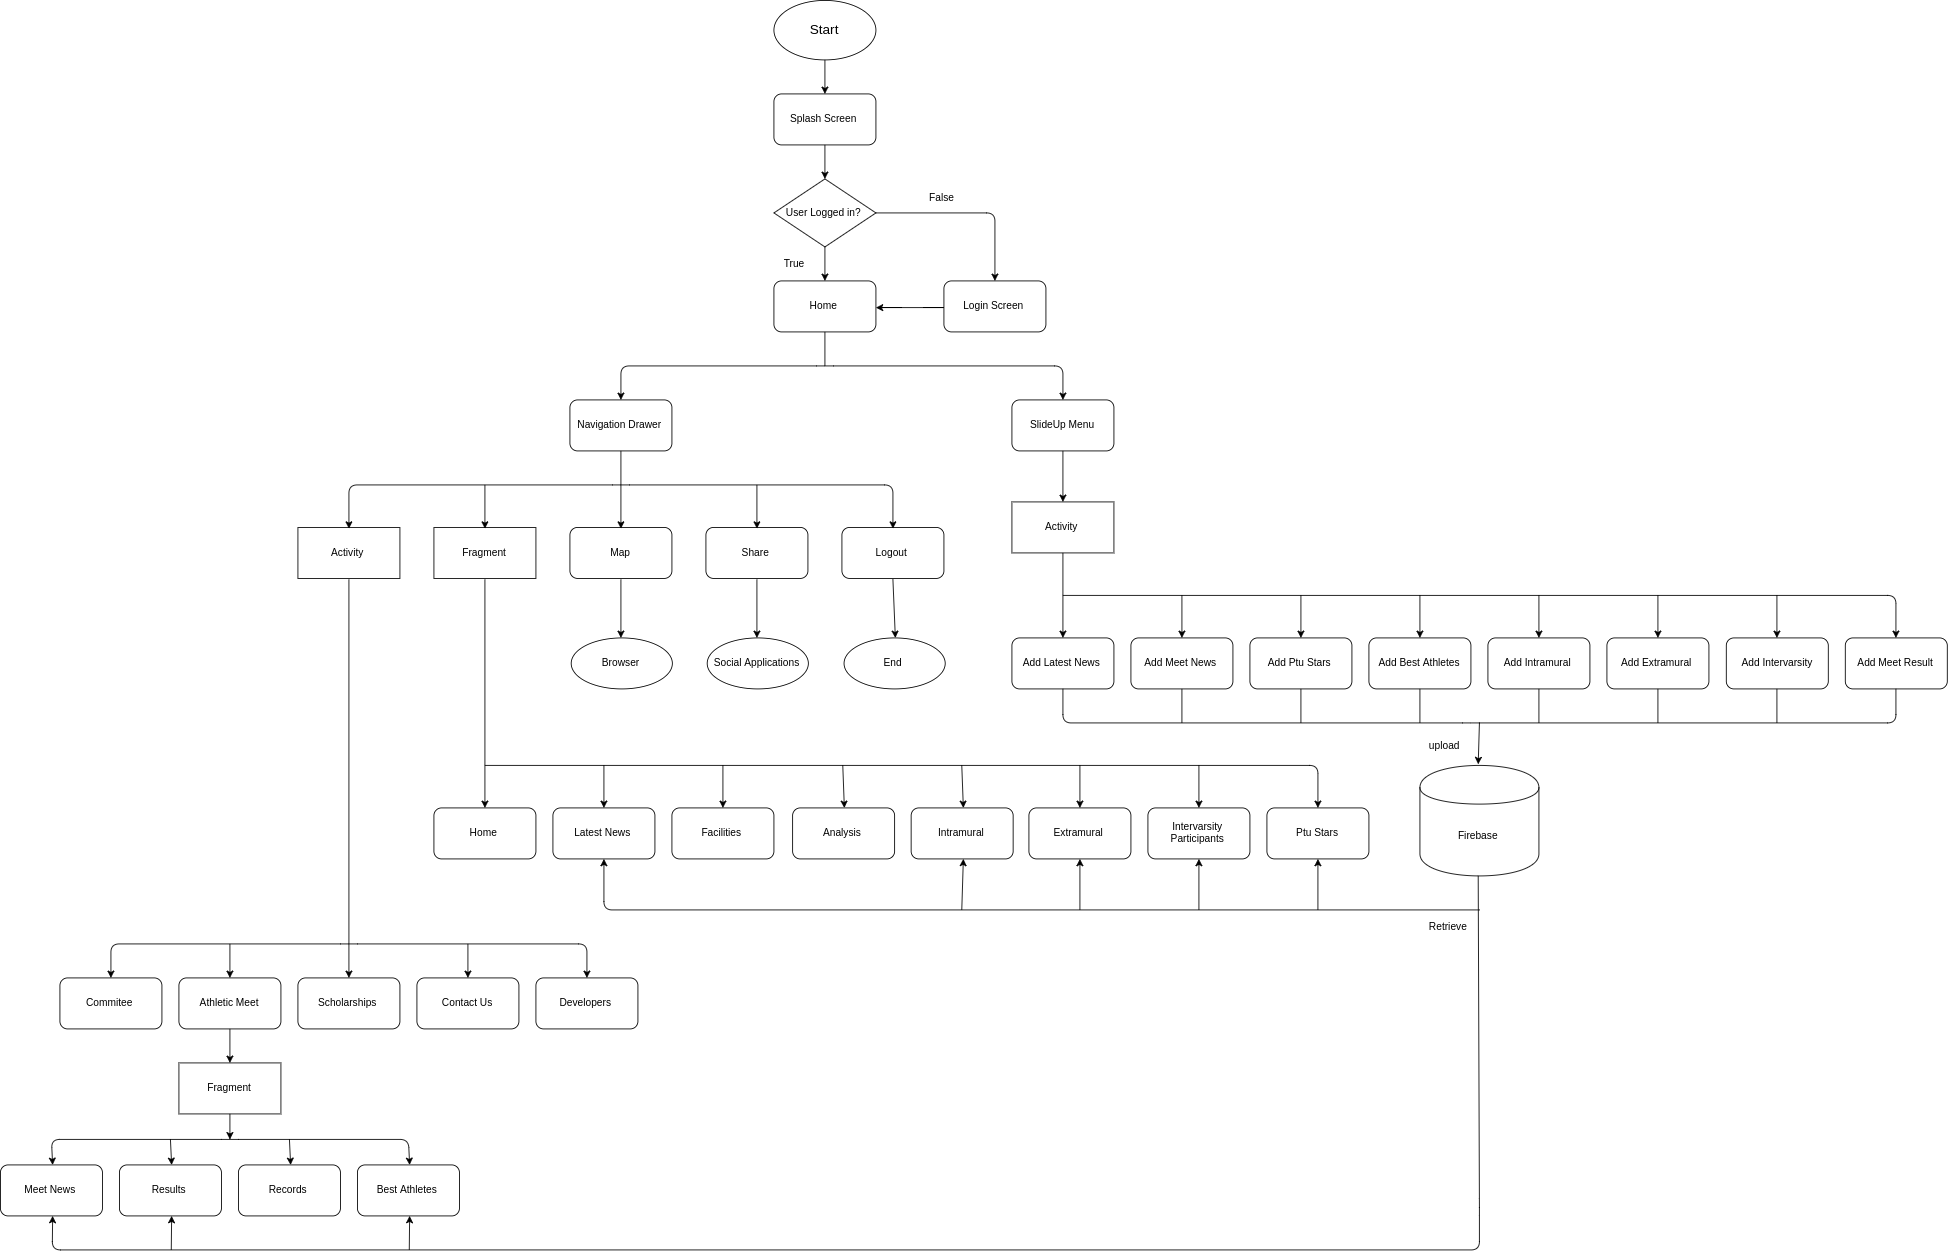
\includegraphics[scale=0.26]{images/Gndecadmingne.png}
	\caption{Flow Chart of gndec admin}
\end{figure}

\newpage
\begin{figure}[ht]
	
	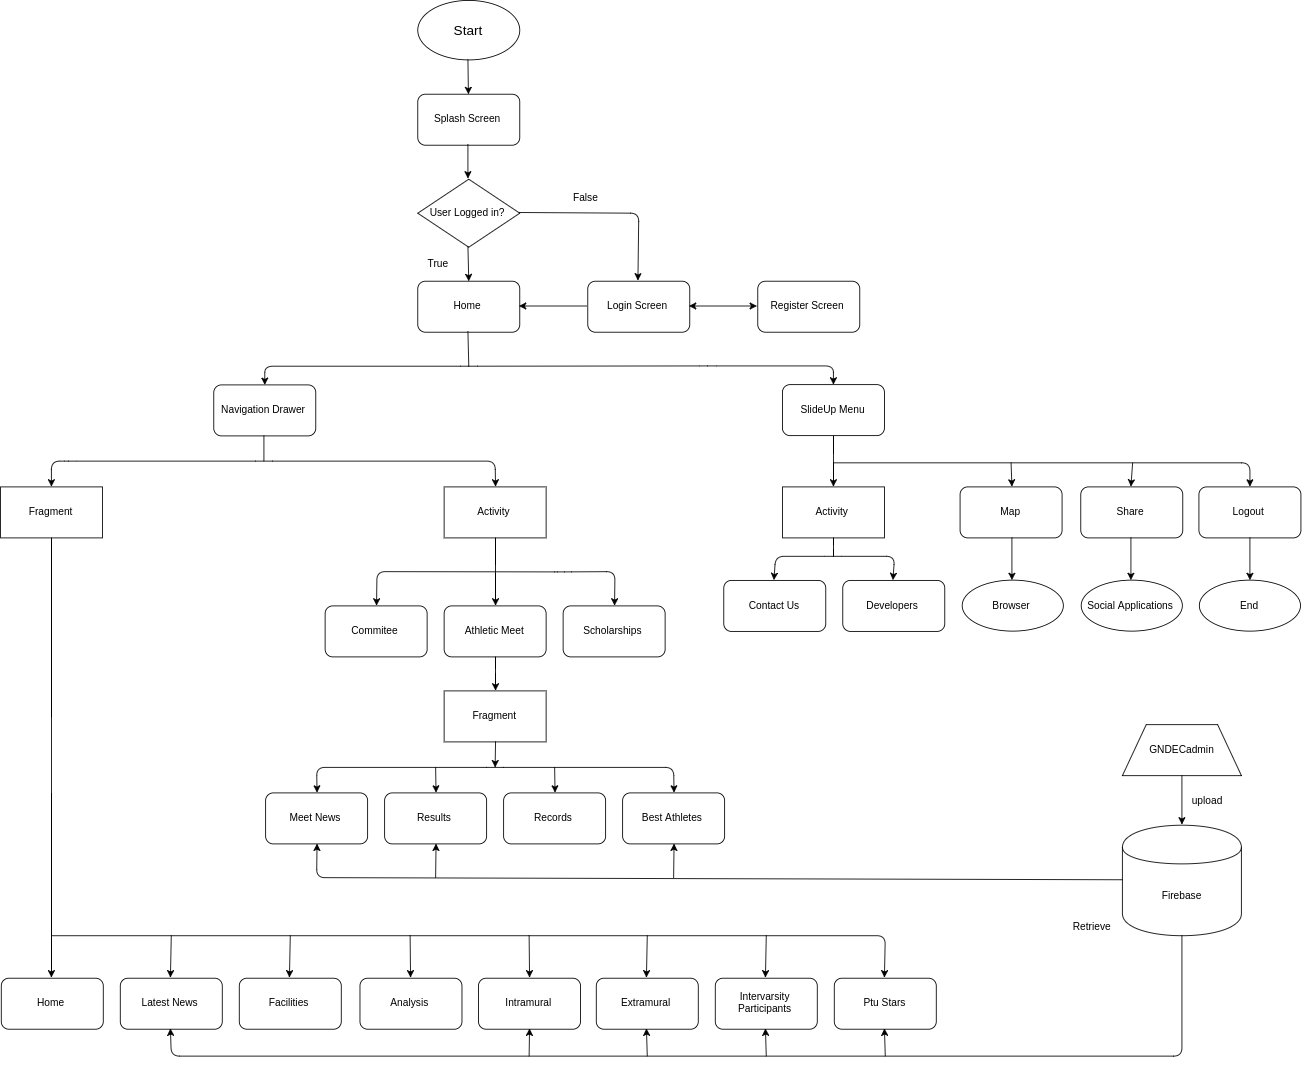
\includegraphics[scale=0.35]{images/Gndecstudent.png}
	\caption{Flow Chart of gndec student}
\end{figure}



\newpage
\section{Database Design}

	\subsection{ER Diagram}
	
	
	\begin{figure}[ht]
		\centering
		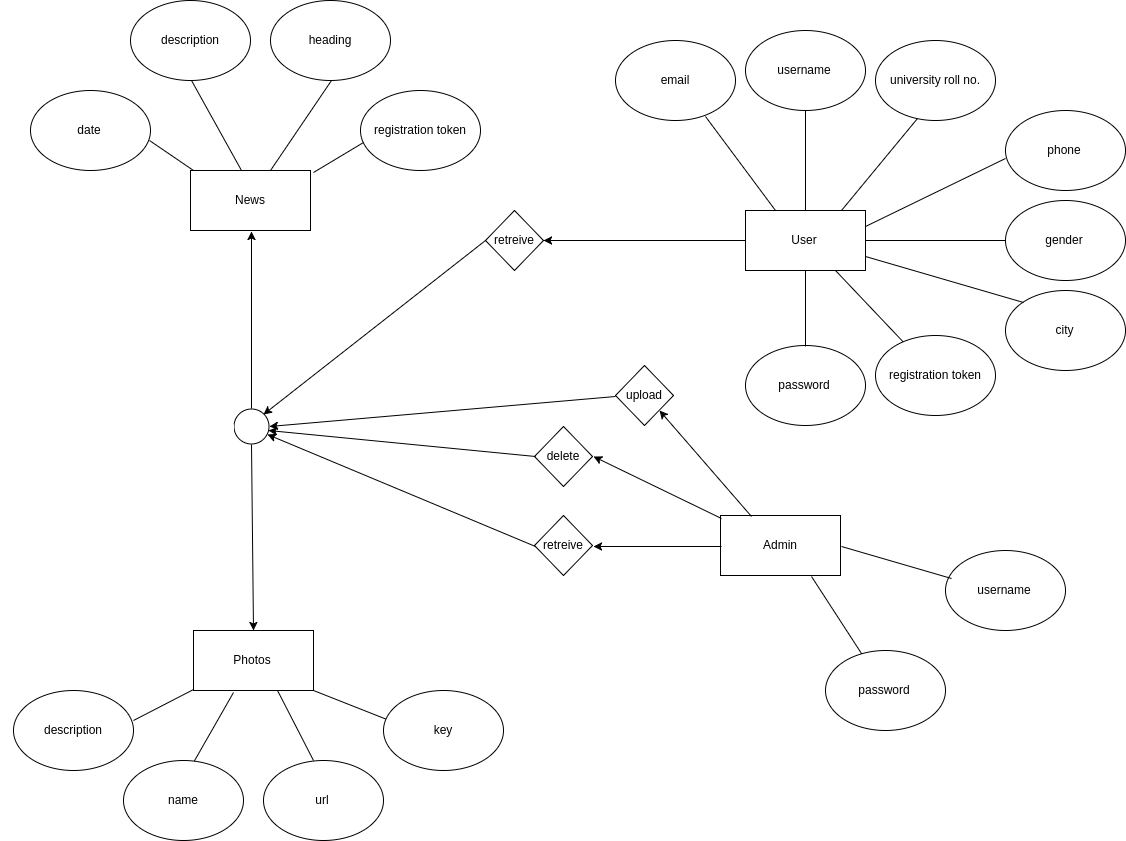
\includegraphics[scale=0.35]{images/ergndec.png}
		\caption{ER Diagram}
	\end{figure}
	
	\subsection{Database Connection Controls and Strings}
	The Firebase Realtime Database is a cloud-hosted database. Data is stored as JSON and synchronized in realtime to every connected client. When we build cross-platform apps with our iOS, Android, and JavaScript SDKs, all of our clients share one Realtime Database instance and automatically receive updates with the newest data. \\
	
	It is recommended using the Firebase Assistant to connect your app to Firebase. The Firebase Assistant can connect our existing project or create a new one for us and automatically install any necessary gradle dependencies.\\

	



\chapter{Implementation ,Testing and Maintenance}
\section{Introduction to Languages,IDE’s,Tools and Technologies used for Implementation}
	
\subsection{Technologies used}

\subsubsection{MATLAB}
 MATLAB (matrix laboratory) is a multi-paradigm numerical computing environment. A proprietary programming language developed by MathWorks, MATLAB allows matrix manipulations, plotting of functions and data, implementation of algorithms, creation of user interfaces, and interfacing with programs written in other languages, including C, C++, Java, Fortran and Python.

Although MATLAB is intended primarily for numerical computing, an optional toolbox uses the MuPAD symbolic engine, allowing access to symbolic computing abilities. An additional package, Simulink, adds graphical multi-domain simulation and model-based design for dynamic and embedded systems.

As of 2017, MATLAB has roughly 1 million users across industry and academia. MATLAB users come from various backgrounds of engineering, science, and economics.

\begin{itemize}

\item \textbf{Setting up a project}

To setup our project, user needs to have a opertaion system along with matlab installed in it. Operting system such as windows, linux will be sufficient to perform retinal image detection.

\begin{figure}[ht]
\centering
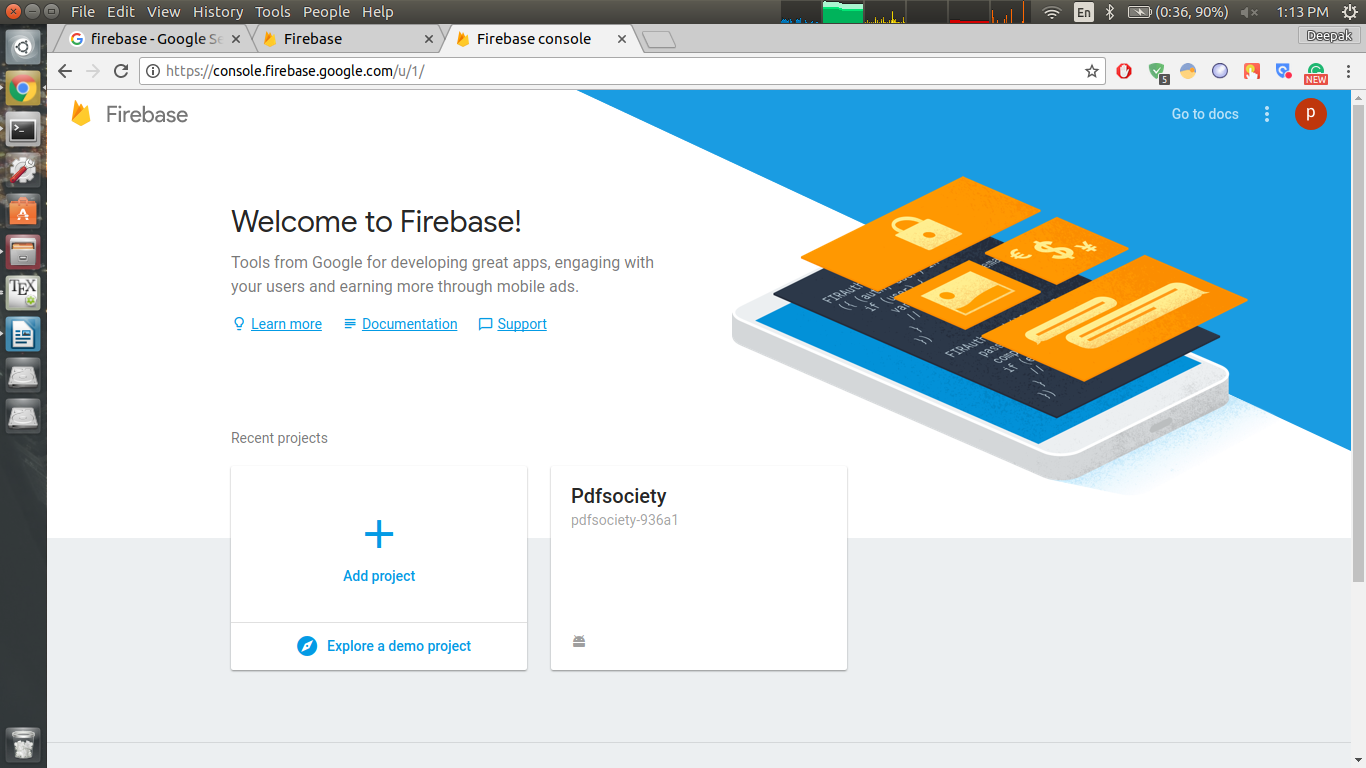
\includegraphics[scale=0.20]{images/Pdf2.png}
\caption{Firebase Console}
\end{figure}

 

\item \textbf{Firebase Products}

\begin{figure}[ht]
\centering
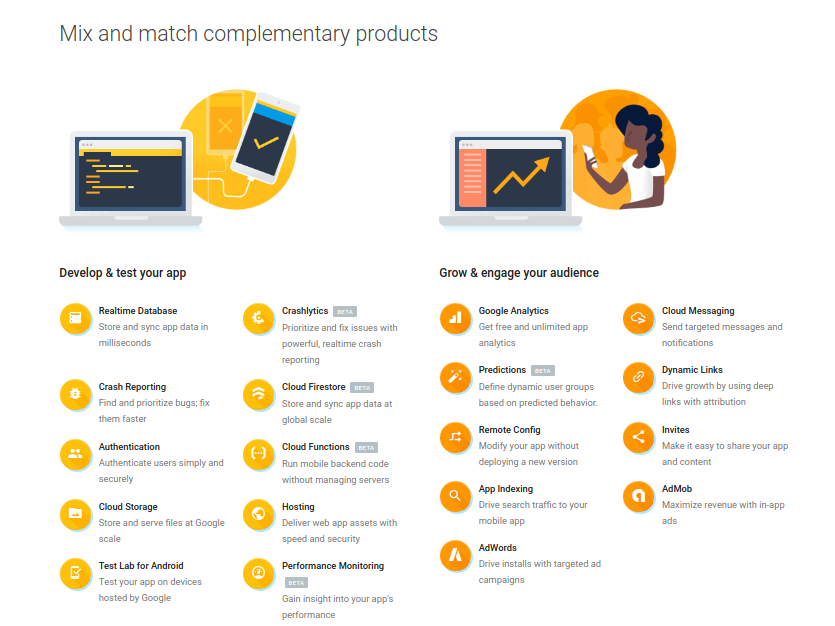
\includegraphics[scale=0.4]{images/Pdf1.png}
\caption{Firebase Products}
\end{figure}

\begin{itemize}

\item \textbf{DRIVE}

The DRIVE database has been established to enable comparative studies on segmentation of blood vessels in retinal images. The research community is invited to test their algorithms on this database and share the results with other researchers through this web site. On this page, instructions can be found on downloading the database and uploading results, and the results of various methods can be inspected. \\

The data included in this database can be used, free of charge, for research and educational purposes. Copying, redistribution, and any unauthorized commercial use is prohibited. The use of this database is restricted to those individuals or organizations that obtained the database directly from this website. Any researcher reporting results which use this database must acknowledge the DRIVE database. We request you to do so by citing this publication:

\item \textbf{Cloud Storage}

Cloud Storage is built for app developers who need to store and serve user-generated content, such as photos or videos.

Cloud Storage for Firebase is a powerful, simple, and cost-effective object storage service built for Google scale. The Firebase SDKs for Cloud Storage add Google security to file uploads and downloads for your Firebase apps, regardless of network quality. You can use our SDKs to store images, audio, video, or other user-generated content. On the server, you can use Google Cloud Storage, to access the same files.
	\end{itemize}
	\end{itemize}
	
\subsubsection{Web Technology}


Web technology is a broad term for the work involved in developing a web site for the Internet (World Wide Web) or an intranet (a private network). Web development can range from developing the simplest static single page of plain text to the most complex web-based internet applications (or just 'web apps') electronic businesses, and social network services. A more comprehensive list of tasks to which web development commonly refers, may include web engineering, web design, web content development, client liaison, client-side/server-side scripting, web server and network security configuration, and e-commerce development. Among web professionals, "web development" usually refers to the main non-design aspects of building web sites: writing markup and coding. 

\begin{figure}[ht]
\centering
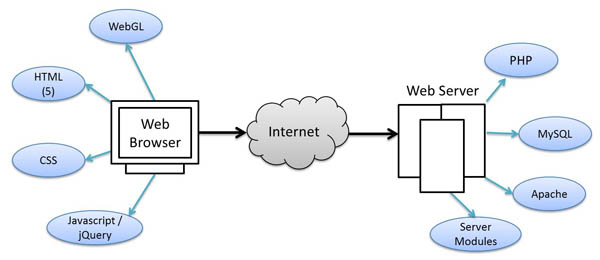
\includegraphics[scale=0.48]{images/WebTechnology.jpg}
\caption{Web Development Anatomy}
\label{fig:Anatomy}
\end{figure}

Most recently Web development has come to mean the creation of content management systems or CMS. These CMS can be made from scratch, proprietary or open source. In broad terms the CMS acts as middleware between the database and the user through the browser. A principle benefit of a CMS is that it allows non-technical people to make changes to their web site without having technical knowledge.

For larger organizations and businesses, web development teams can consist of hundreds of people (web developers) and follow standard methods like Agile methodologies while developing websites. Smaller organizations may only require a single permanent or contracting developer, or secondary assignment to related job positions such as a graphic designer or information systems technician. Web development may be a collaborative effort between departments rather than the domain of a designated department. There are three kinds of web developer specialization: front-end developer, back-end developer, and full-stack developer. Front-end developers deal with the layout and visuals of a website, while back-end developers deal with the functionality of a website. Back-end developers will program in the functions of a website that will collect data.
Since the commercialization of the web, web development has been a growing industry. The growth of this industry is being driven by businesses wishing to use their website to sell products and services to customers.[1]

There is open source software for web development like BerkeleyDB, GlassFish, LAMP (Linux, Apache, MySQL, PHP) stack and Perl/Plack. This has kept the cost of learning web development to a minimum. Another contributing factor to the growth of the industry has been the rise of easy-to-use WYSIWYG web-development software, such as Adobe Dreamweaver, BlueGriffon and Microsoft Visual Studio. Knowledge of HyperText Markup Language (HTML) or of programming languages is still required to use such software, but the basics can be learned and implemented quickly with the help of help files, technical books, internet tutorials, or face-to-face training.



\begin{itemize}

\item \textbf{Activity Lifecycle}
Activities in the system are managed as an activity stack. When a new activity
is started, it is placed on the top of the stack and becomes the running activitythe previous activity always remains below it in the stack, and will not come to
the foreground again until the new activity exits. An activity has essentially four
states:
If an activity in the foreground of the screen (at the top of the stack), it is
active or running.

If an activity has lost focus but is still visible (that is, a new non-full-sized or
transparent activity has focus on top of your activity), it is paused. A paused
activity is completely alive (it maintains all state and member information and
remains attached to the window manager), but can be killed by the system in
extreme low memory situations.


\end{itemize}

\subsection{Language used}
\subsubsection{FORTAN}

Fortran
Fortran acs cover.jpeg
The Fortran Automatic Coding System for the IBM 704 (15 October 1956), the first Programmer's Reference Manual for Fortran
Paradigm	multi-paradigm: structured, imperative (procedural, object-oriented), generic
Designed by	John Backus
Developer	John Backus and IBM
First appeared	1957; 61 years ago
Stable release	
Fortran 2008 (ISO/IEC 1539-1:2010) / 2010; 8 years ago
Typing discipline	strong, static, manifest
Filename extensions	.f, .for, .f90
Major implementations
Absoft, Cray, GFortran, G95, IBM XL Fortran, Intel, Hitachi, Lahey/Fujitsu, Numerical Algorithms Group, Open Watcom, PathScale, PGI, Silverfrost, Oracle Solaris Studio, Visual Fortran, others
Influenced by
Speedcoding
Influenced
ALGOL 58, BASIC, C, Chapel,[1] CMS-2, Fortress, PL/I, PACT I, MUMPS and Ratfor
Fortran (/ˈfɔːrtræn/; formerly FORTRAN, derived from Formula Translation[2]) is a general-purpose, imperative programming language that is especially suited to numeric computation and scientific computing. Originally developed by IBM[3] in the 1950s for scientific and engineering applications, FORTRAN came to dominate this area of programming early on and has been in continuous use for over half a century in computationally intensive areas such as numerical weather prediction, finite element analysis, computational fluid dynamics, computational physics, crystallography and computational chemistry. It is a popular language for high-performance computing[4] and is used for programs that benchmark and rank the world's fastest supercomputers.[5]

Fortran encompasses a lineage of versions, each of which evolved to add extensions to the language while usually retaining compatibility with prior versions. Successive versions have added support for structured programming and processing of character-based data (FORTRAN 77), array programming, modular programming and generic programming (Fortran 90), high performance Fortran (Fortran 95), object-oriented programming (Fortran 2003) and concurrent programming (Fortran 2008).

The characteristics and features of java are as follows :

\begin{itemize}
	\item 

Matlab is easy to understand because of its user interface. It has a very friendly user interface.  


\item The main reason is that Matlab is dynamically typed. That is, a variable can change type as it is modified.


\begin{itemize}
	\item Functional programming language
	
\item Support for objects

\end{itemize}

\item \textbf{Secure}
Matlab is Secure Language because of its many features it enables to
develop virus-free, tamper-free systems. Authentication techniques are
based on public-key encryption.

\item \textbf{Robust}

Robust Javascript was created as a strongly typed language. Data type issues
and problems are resolved at compile-time, and implicit casts of a variable
from one type to another are not allowed.

\item \textbf{Architectural Neural}
Architecture neutral It is not easy to write an application that can be used
on Windows , UNIX and a Macintosh. And its getting more complicated
with the move of windows to non Intel CPU architectures.
matlab takes a diffierent approach. 
\item \textbf{Portable}
Portable matlab code is portable. It was an important design goal of Javascript that it
be portable so that as new architectures(due to hardware, operating system,
or both)

\item \textbf{High performance}
High performance For all but the simplest or most infrequently used appli-cations,
performance is always a consideration for most applications, including
21graphics-intensive ones such as are commonly found on the world wide web,
the performance of matlab is more than adequate.



\end{itemize}

\subsection{IDE used}
\subsubsection{Matlab}

\begin{figure}[ht]
\centering

\includegraphics[scale=0.90]{images/VisualStudio.png}
\caption{Visual Studio}
\end{figure}

MATLAB (matrix laboratory) is a multi-paradigm numerical computing environment. A proprietary programming language developed by MathWorks, MATLAB allows matrix manipulations, plotting of functions and data, implementation of algorithms, creation of user interfaces, and interfacing with programs written in other languages, including C, C++, Java, Fortran and Python.\\
Although MATLAB is intended primarily for numerical computing, an optional toolbox uses the MuPAD symbolic engine, allowing access to symbolic computing abilities. An additional package, Simulink, adds graphical multi-domain simulation and model-based design for dynamic and embedded systems.

As of 2017, MATLAB has roughly 1 million users across industry and academia. MATLAB users come from various backgrounds of engineering, science, and economics





\begin{itemize}
\item \textbf{System Requirements}
Web application development on either of the following operating systems −
\vskip 0.1in

Microsoft Windows 10/8/7/Vista/2003 (32 or 64-bit)
\\Mac OS X 10.8.5 or higher, up to 10.9 (Mavericks)
\\GNOME or KDE desktop
\vskip 0.1in

\end{itemize}

\subsection{Introduction to \LaTeX}
\begin{figure}[ht]
\centering
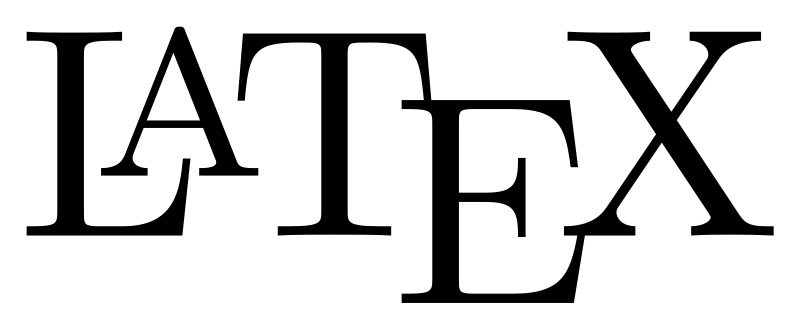
\includegraphics[scale=0.2]{images/latex.png}
\caption{\LaTeX{} Logo}
\end{figure}
\hspace{-1.8em} \LaTeX{}, I had never heard about this term before doing this project,
but when I came to know about it's features, it is just excellent. 
\LaTeX (pronounced /ˈleɪtɛk/, /ˈleɪtɛx/, /ˈlɑːtɛx/, or /ˈlɑːtɛk/) is a 
document markup language and document preparation system for the \TeX{} 
typesetting  program. Within the typesetting system, its name is styled 
as \LaTeX.

\hspace{-1.8em} Within the typesetting system, its name is styled as \LaTeX. The term 
\LaTeX{} refers only to the language in which documents are written, 
not to the editor used to write those documents. In order to create a 
document in \LaTeX, a .tex file must be created using some form of text 
editor. While most text editors can be used to create a \LaTeX{} document, 
a number of editors have been created specifically for working with \LaTeX.\\

\noindent\LaTeX{} is most widely used by mathematicians, scientists, 
engineers, philosophers, linguists, economists and other scholars in 
academia. As a primary or intermediate format, e.g., translating DocBook 
and other XML-based formats to PDF, \LaTeX{} is used because of the 
high quality of typesetting achievable by \TeX. The typesetting system 
offers programmable desktop publishing features and extensive facilities 
for automating most aspects of typesetting and desktop publishing, 
including numbering and cross-referencing, tables and figures, 
page layout and bibliographies.\\

\noindent\LaTeX{} is intended to provide a high-level language that
accesses the power of \TeX. \LaTeX{} essentially comprises a
collection of \TeX{} macros and a program to process \LaTeX documents. 
Because the \TeX{} formatting commands are very low-level, it is usually 
much simpler for end-users to use \LaTeX{}.


\subsubsection{Typesetting}
\LaTeX{} is based on the idea that authors should be able to focus on 
the content of what they are writing without being distracted by its 
visual presentation. in preparing a \LaTeX{} document, the author 
specifies the logical structure using familiar concepts such as 
chapter, section, table, figure, etc., and lets the \LaTeX{} system 
worry about the presentation of these structures. it therefore 
encourages the separation of layout from content while still allowing 
manual typesetting adjustments where needed. 

\begin{verbatim}
\documentclass[12pt]{article}
\usepackage{amsmath}
\title{\LaTeX}
\begin{document}
  \maketitle 
  \LaTeX{} is a document preparation system 
  for the \TeX{} typesetting program.
   \par 
   $E=mc^2$
\end{document}
\end{verbatim}

\subsubsection{Installing \LaTeX{} on System}
Installation of \LaTeX{} on personal system is quite easy. As i have used \LaTeX{} on Ubuntu 13.04 so i am discussing the installation steps for Ubuntu 13.04 here:
\begin{itemize}
\item Go to terminal and type\\\\
\textit{sudo apt-get install texlive-full}
\item Your Latex will be installed on your system and you can check for manual page by typing.\\\\
\textit{man latex}\\

in terminal which gives manual for latex command.
\item To do very next step now one should stick this to mind that the document which one is going to produce is written in any type of editor whether it may be your most common usable editor Gedit or you can use vim by installing first vim into your system using command.\\\\
\textit{sudo apt-get install vim}
\item After you have written your document it is to be embedded with some set of commands that Latex uses so as to give a structure to your document. Note that whenever you wish your document to be looked into some other style just change these set of commands.
\item When you have done all these things save your piece of code with .tex format say test.tex. Go to terminal and type\\\\
\textit{latex path of the file test.tex Or pdflatex path of the file test.tex\\ eg: pdflatex test.tex}\\
for producing pdf file simultaneously.\\
After compiling it type command\\\\
\textit{evince filename.pdf\\ eg: evince test.pdf}\\
To see output pdf file. 
\end{itemize}
\subsubsection{Pdfscreen \LaTeX{}}
There are some packages that can help to have unified document using \LaTeX{}. Example of such a package is pdfscreen that let the user view it’s document in two forms-print and screen. Print for hard copy and screen for viewing your document on screen. Download this package from www.ctan.org/tex-archive/macros/latex/contrib/pdfscreen/.\\
Then install it using above mention method.\\

\noindent To test it the test code is given below:-\\
Just changing print to screen gives an entirely different view. But for working of pdfscreen another package required are comment and fancybox.\\

\noindent The fancybox package provides several different styles of boxes for framing and rotating content in your document. Fancybox provides commands that produce square-cornered boxes with single or double lines, boxes with shadows, and round-cornered boxes with normal or bold lines. You can box mathematics, floats, center, flushleft, and flushright, lists, and pages.\\
 	
\noindent Whereas comments package selectively include/excludes portions of text. The comment package allows you to declare areas of a document to be included or excluded. One need to make these declarations in the preamble of your file. The package uses a method for exclusion that is pretty robust, and can cope with ill-formed bunches of text.\\

\noindent So these extra packages needed to be installed on system for the proper working of pdfscreen package.


	\section{Coding standards of Language used 
}

\subsection{Coding standards for Javascript }
\begin{itemize}

\item Preprocessor Where the use of a language preprocessor is required, it will be the C preprocessor (cpp). cpp is available on any UNIX platform, and many Fortran compilers have the ability to run cpp automatically as part of the compilation process. All tokens will be uppercase to distinguish them from Fortran code, which will be in lower case.

\item F90 Standard CCM4 will adhere to the Fortran 90 language standard. The purpose is to enhance portability, and to allow use of the many desirable new features of the language. If a situation arises in which there is good reason to violate this rule and include Fortran code which is not compliant with the f90 standard, an alternate set of f90-compliant code must be provided. This is normally done through use of a C-preprocessor ifdef construct.
\item Lines should usually be no longer than 80 characters, and should not exceed 100 (counting tabs as 4 spaces). This is a “soft” rule, but long lines generally indicate unreadable or disorganized code.
\item Loops Loops should be structured with the do-end do construct as opposed to numbered loops.
\item Unary special-character operators (e.g., ++, --) must not have space next to their operand.
\item Any, and; must not have preceding space.
\item Any; used as a statement terminator must be at the end of the line.
\item Any: after a property name in an object definition must not have preceding space.
\item The? and: in a ternary conditional must have space on both sides.
\item No filler spaces in empty constructs (e.g., {}, [], fn ()).
.


\end{itemize}

	\section{GANTT chart
	}
	\begin{figure}[ht]
\centering
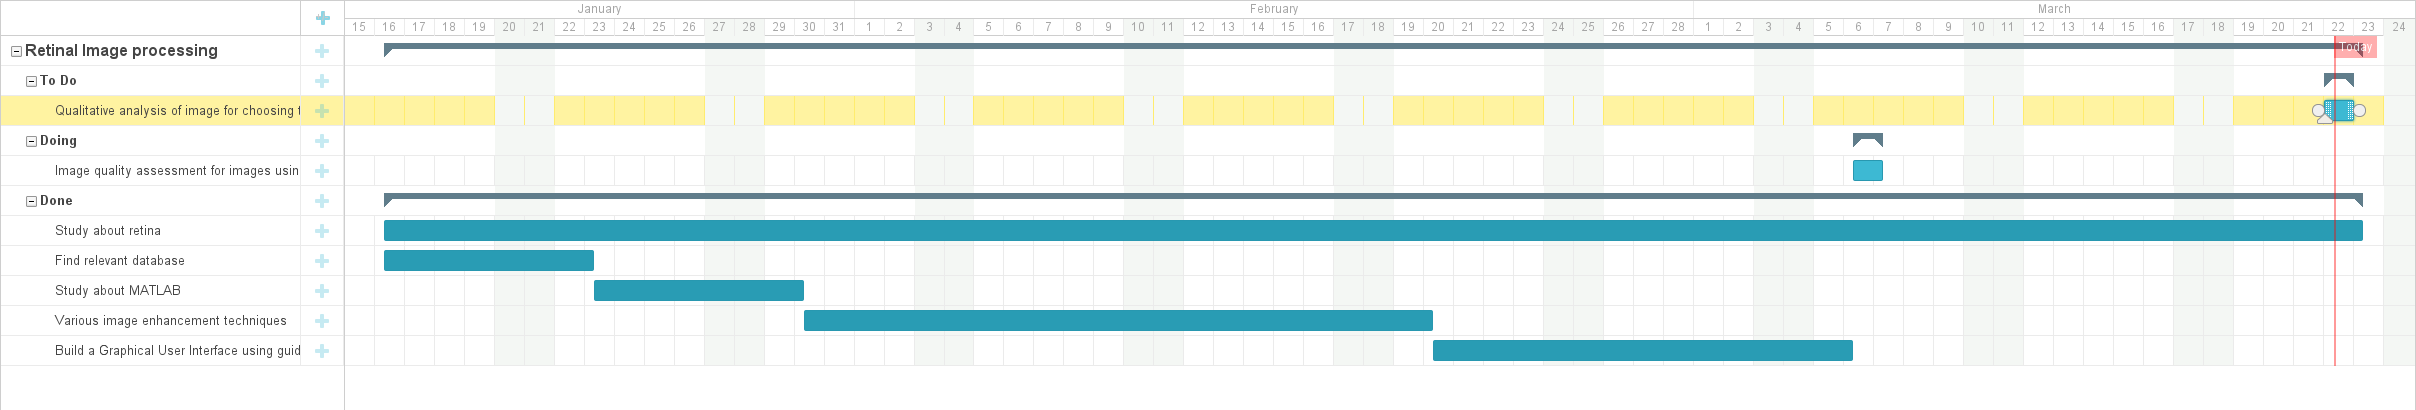
\includegraphics[scale=0.20]{images/GantChart.png}
\caption{\LaTeX{} Ghant chart}
\end{figure}
	
	\section{Testing Techniques and Test Plans
}
\subsection{Functionality Testing}
Test for – all the links in desktop application, 
submitting or getting information from user, cookie testing.

\subsection{Usability testing}
Web site should be easy to use. Instructions should be provided clearly. Check if the provided
instructions are correct meaning whether they satisfy the purpose. Main menu should be
provided on each page. It should be consistent.


\subsection{Compatibility Testing}
Compatibility of your web site is very important testing aspect. See which compatibility test is
to be executed:
\\i. Operating system compatibility
\\ii. Computer processing compatibility

\subsection{Performance Testing}
Desktop application should sustain to heavy load. Desktop performance testing should include:
\\i. Load Testing
\\ii. Stress Testing




\chapter{Results and Discussions}
\section{User Interface Representation (Of  Respective Project)}

The applications interface is designed for retinal image enhancement, the functionality is implemented using matlab, and the phase of testing the product was accomplished successfully. The application can very well manage by the medical staff .
Also doctors can detect the early disease in a human body using enhanced retinal image delivered by our project .
  



\subsection{Snapshots of system}


\begin{figure}[ht]
\centering
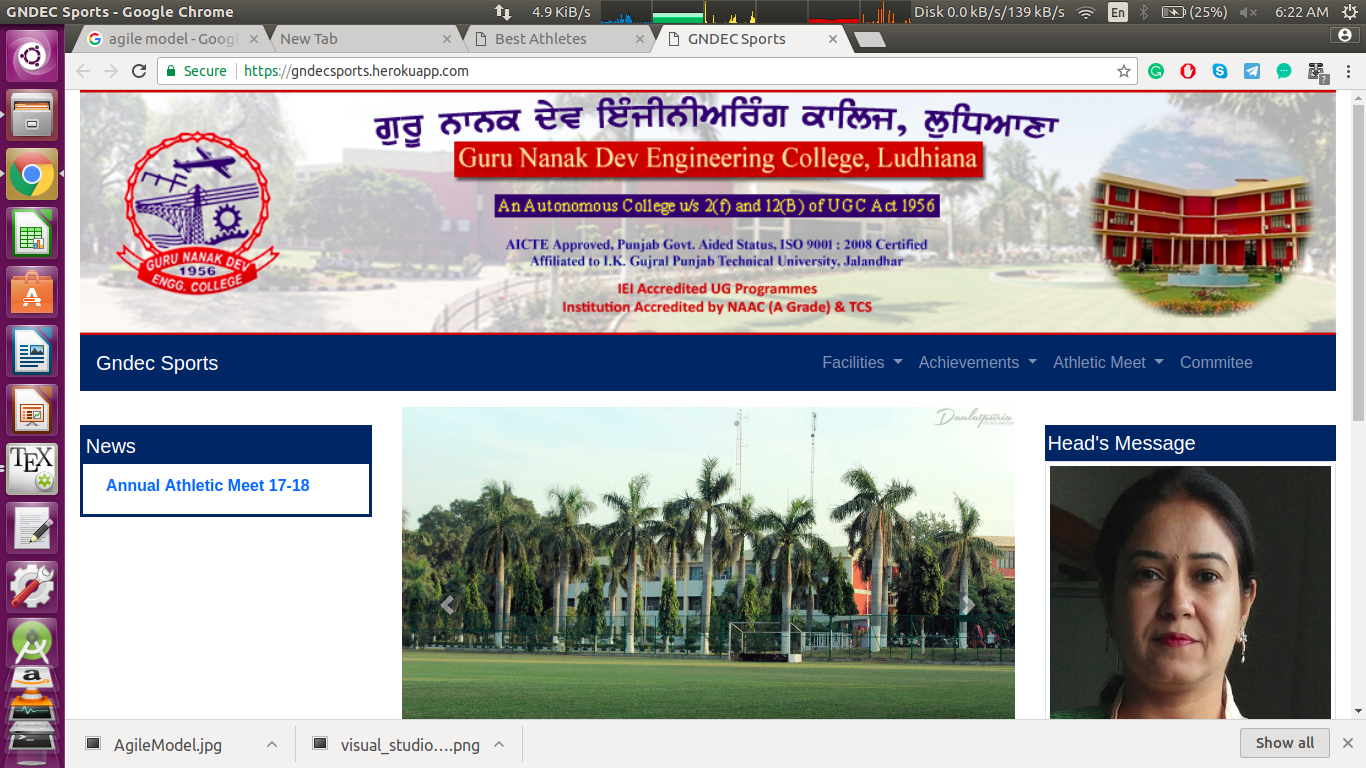
\includegraphics[scale=0.28]{images/HomeUserHeroku.png}
\caption{Home Screen}
\end{figure}

\newpage
\begin{figure}[ht]
\centering
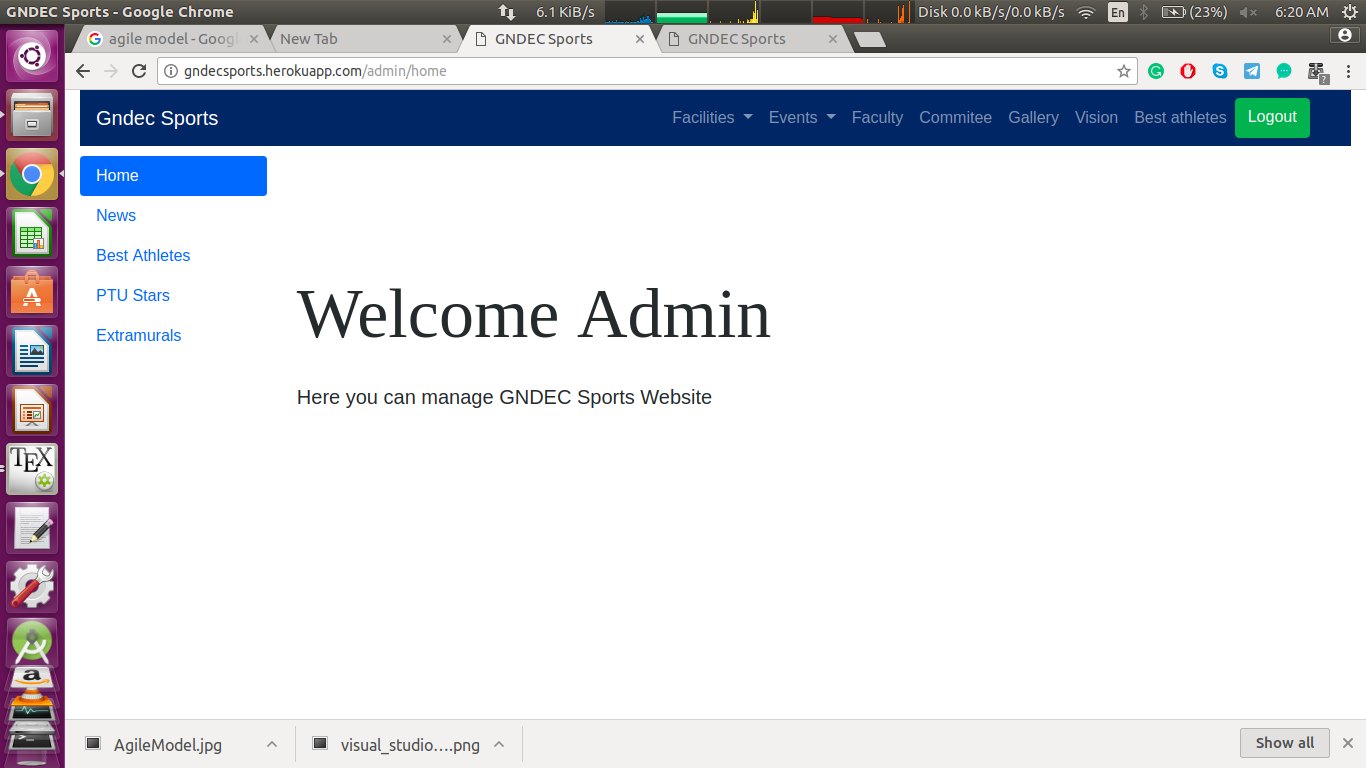
\includegraphics[scale=0.35]{images/HomeAdminHeroku.png}
\caption{Home Screen (Admin)}
\end{figure}

\newpage

\begin{figure}[ht]
\centering
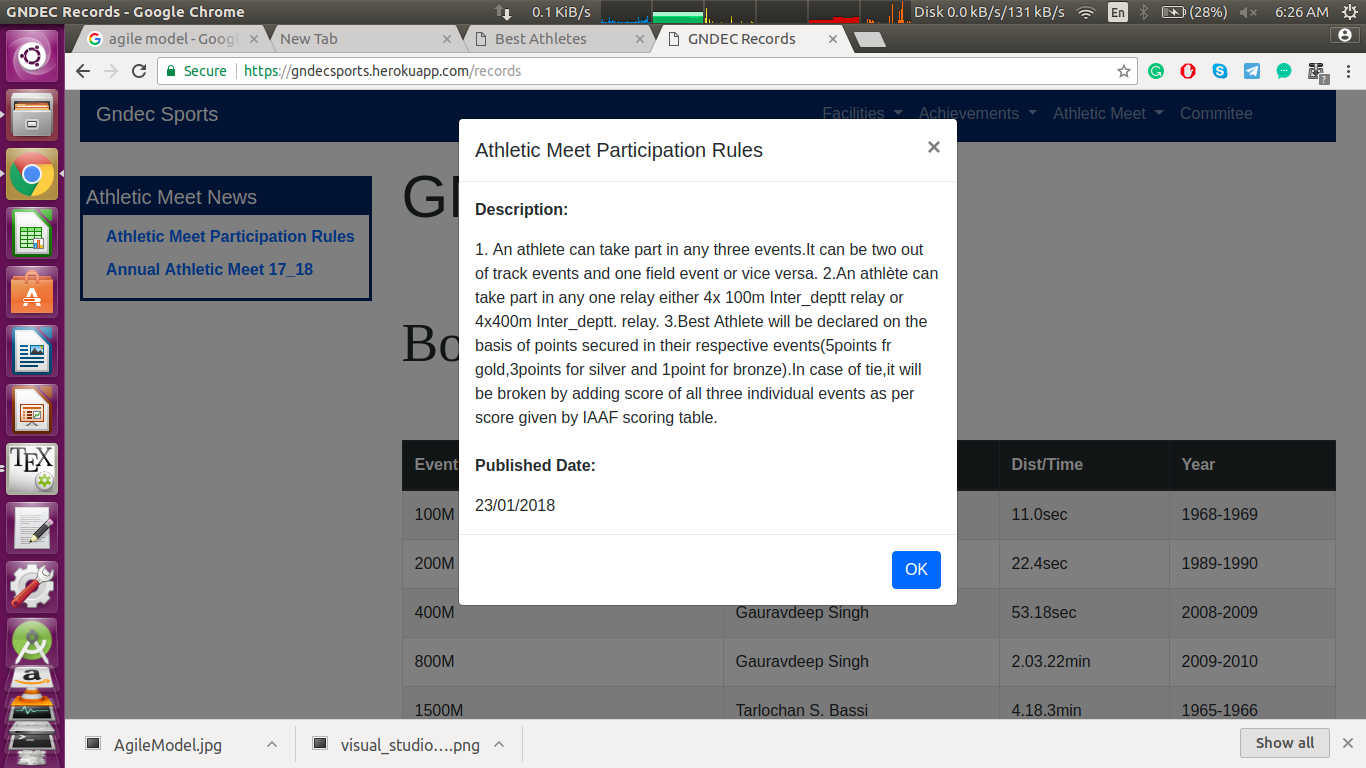
\includegraphics[scale=0.35]{images/NewsPanelHeroku.png}
\caption{News Panel}
\end{figure}

\newpage

\begin{figure}[ht]
\centering
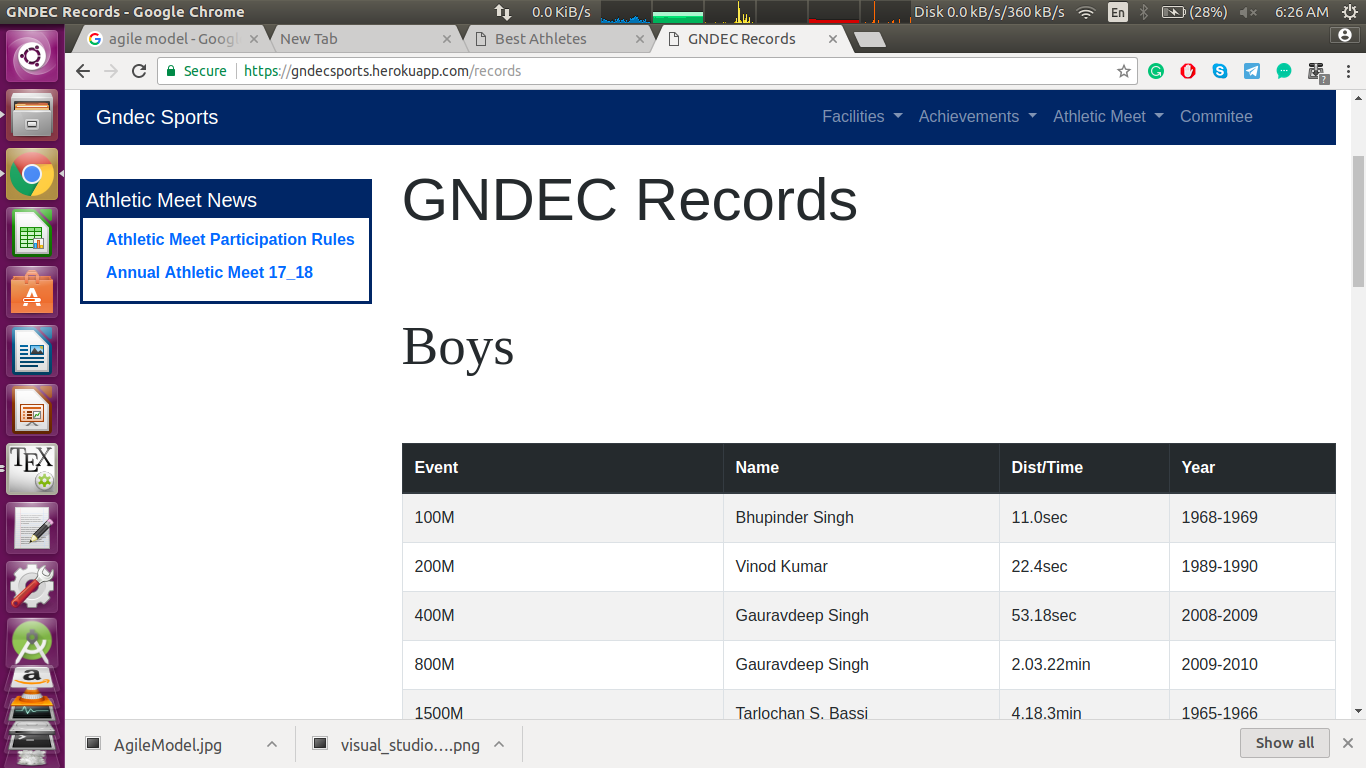
\includegraphics[scale=0.35]{images/RecordsHeroku.png}
\caption{Records}
\end{figure}

\newpage

\begin{figure}[ht]
\centering
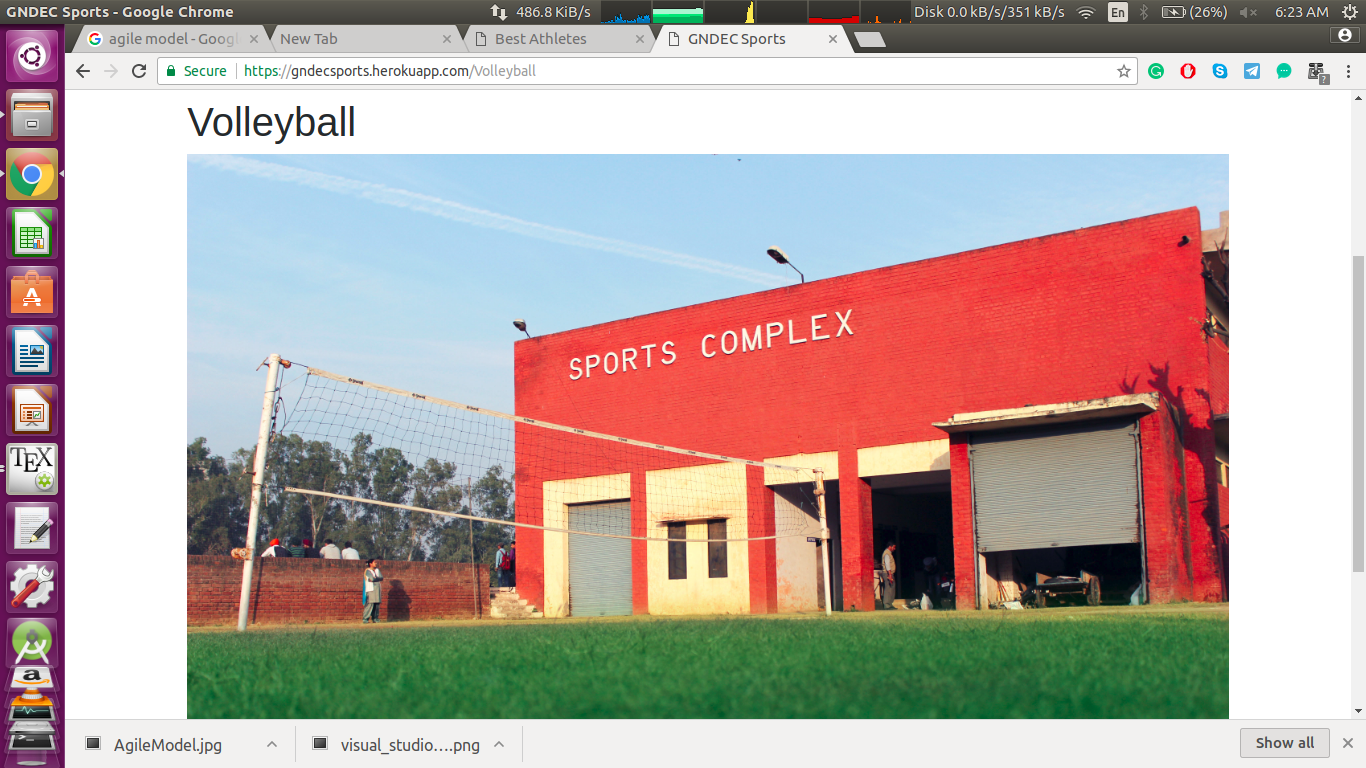
\includegraphics[scale=0.35]{images/VollyballHeroku.png}
\caption{Facilities}
\end{figure}

\newpage

\begin{figure}[ht]
\centering
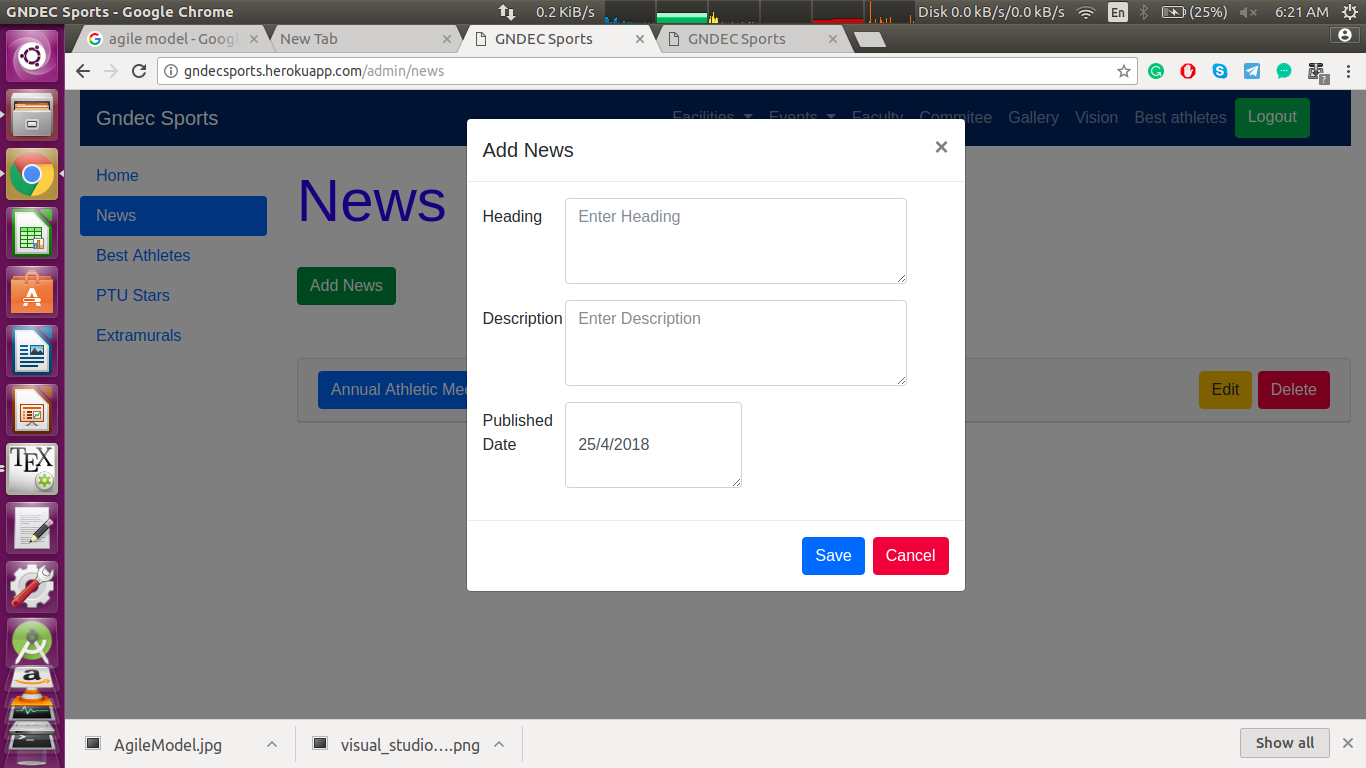
\includegraphics[scale=0.35]{images/AddNewsHeroku.png}
\caption{Add News Panel}
\end{figure}

\newpage

\begin{figure}[ht]
\centering
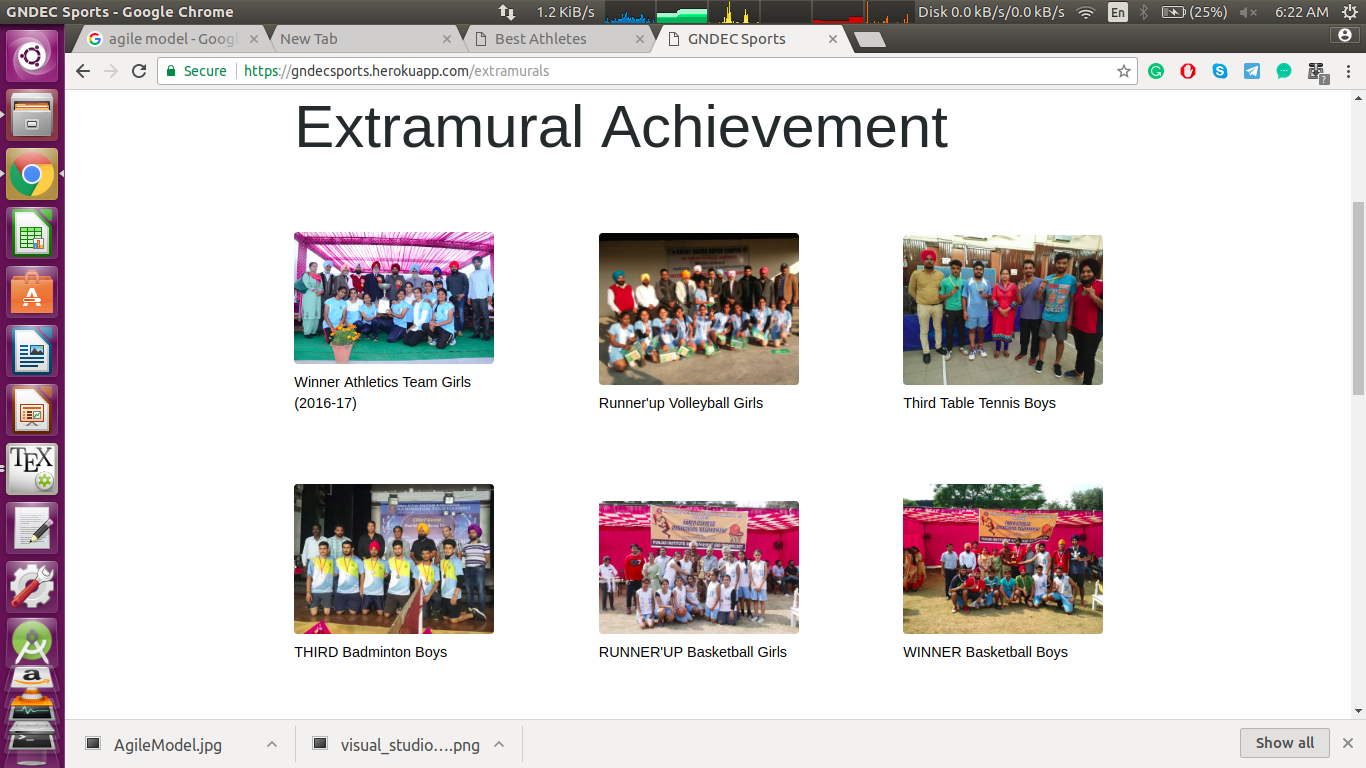
\includegraphics[scale=0.35]{images/AchievementHeroku.png}
\caption{Achievements}
\end{figure}

\newpage

\begin{figure}[ht]
\centering
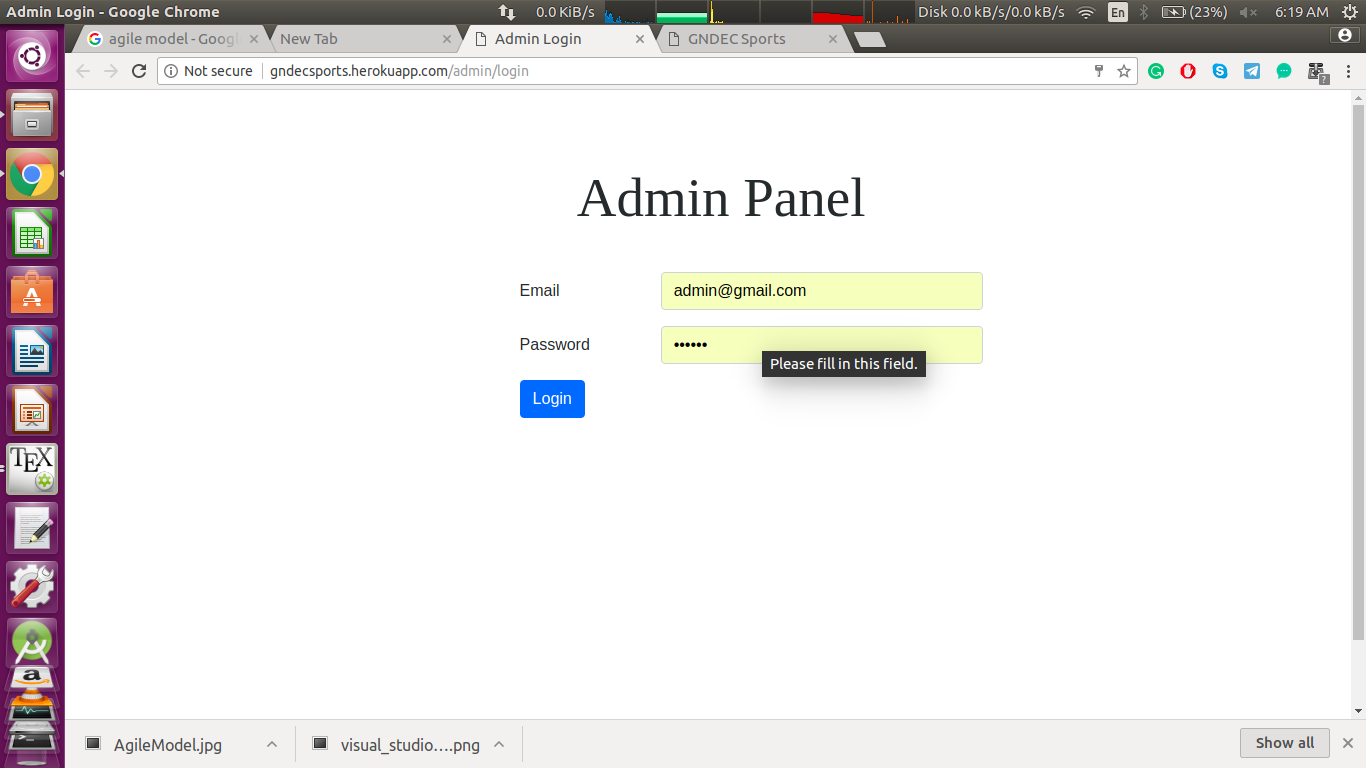
\includegraphics[scale=0.35]{images/AdminPanelHeroku.png}
\caption{Admin Login Panel}
\end{figure}

\newpage

\begin{figure}[ht]
\centering
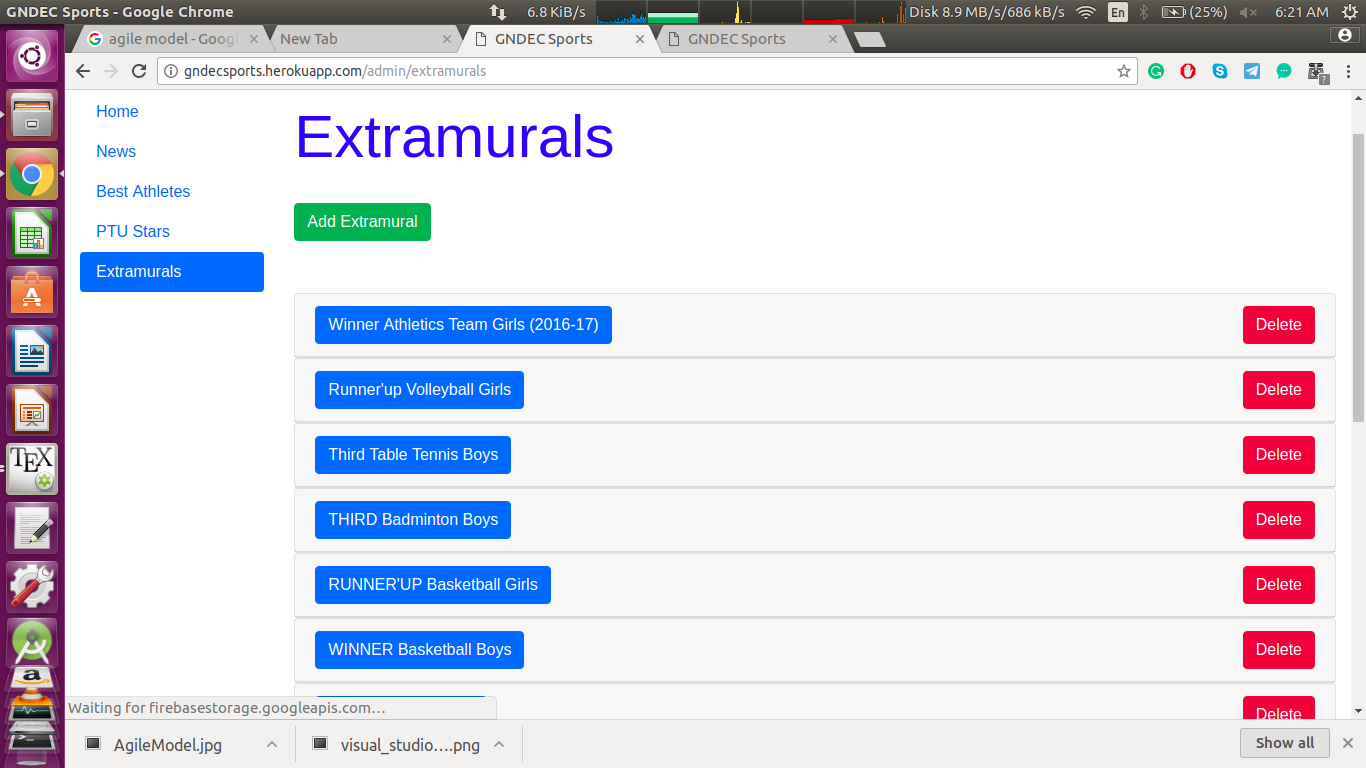
\includegraphics[scale=0.35]{images/ExtramuralHeroku.png}
\caption{Extramural}
\end{figure}


\newpage
\section{Back Ends Representation (Database to be used)}
\subsection{DRIVE}
The photographs for the DRIVE database were obtained from a diabetic retinopathy screening program in The Netherlands. The screening population consisted of 400 diabetic subjects between 25-90 years of age. Forty photographs have been randomly selected, 33 do not show any sign of diabetic retinopathy and 7 show signs of mild early diabetic retinopathy. Each image has been JPEG compressed.

The images were acquired using a Canon CR5 non-mydriatic 3CCD camera with a 45 degree field of view (FOV). Each image was captured using 8 bits per color plane at 768 by 584 pixels. The FOV of each image is circular with a diameter of approximately 540 pixels. For this database, the images have been cropped around the FOV. For each image, a mask image is provided that delineates the FOV.

\subsection{How does it work?}

The set of 40 images has been divided into a training and a test set, both containing 20 images. For the training images, a single manual segmentation of the vasculature is available. For the test cases, two manual segmentations are available; one is used as gold standard, the other one can be used to compare computer generated segmentations with those of an independent human observer. All human observers that manually segmented the vasculature were instructed and trained by an experienced ophthalmologist. They were asked to mark all pixels for which they were for at least 70 percent certain that they were vessel.

All of the images contained in the database were actually used for making clinical diagnoses. To ensure the utmost protection of patient privacy, information that might allow the identity of a patient to be reconstructed has been removed, and we have no actual knowledge that the images could be used alone or in combination to identify any subject. To minimize any further risk of breach of privacy, the use of this database is restricted to those individuals or organizations that obtained the database directly from this website.

\newpage
\subsection{Snapshots of Database}
\begin{figure}[ht]
		\centering
		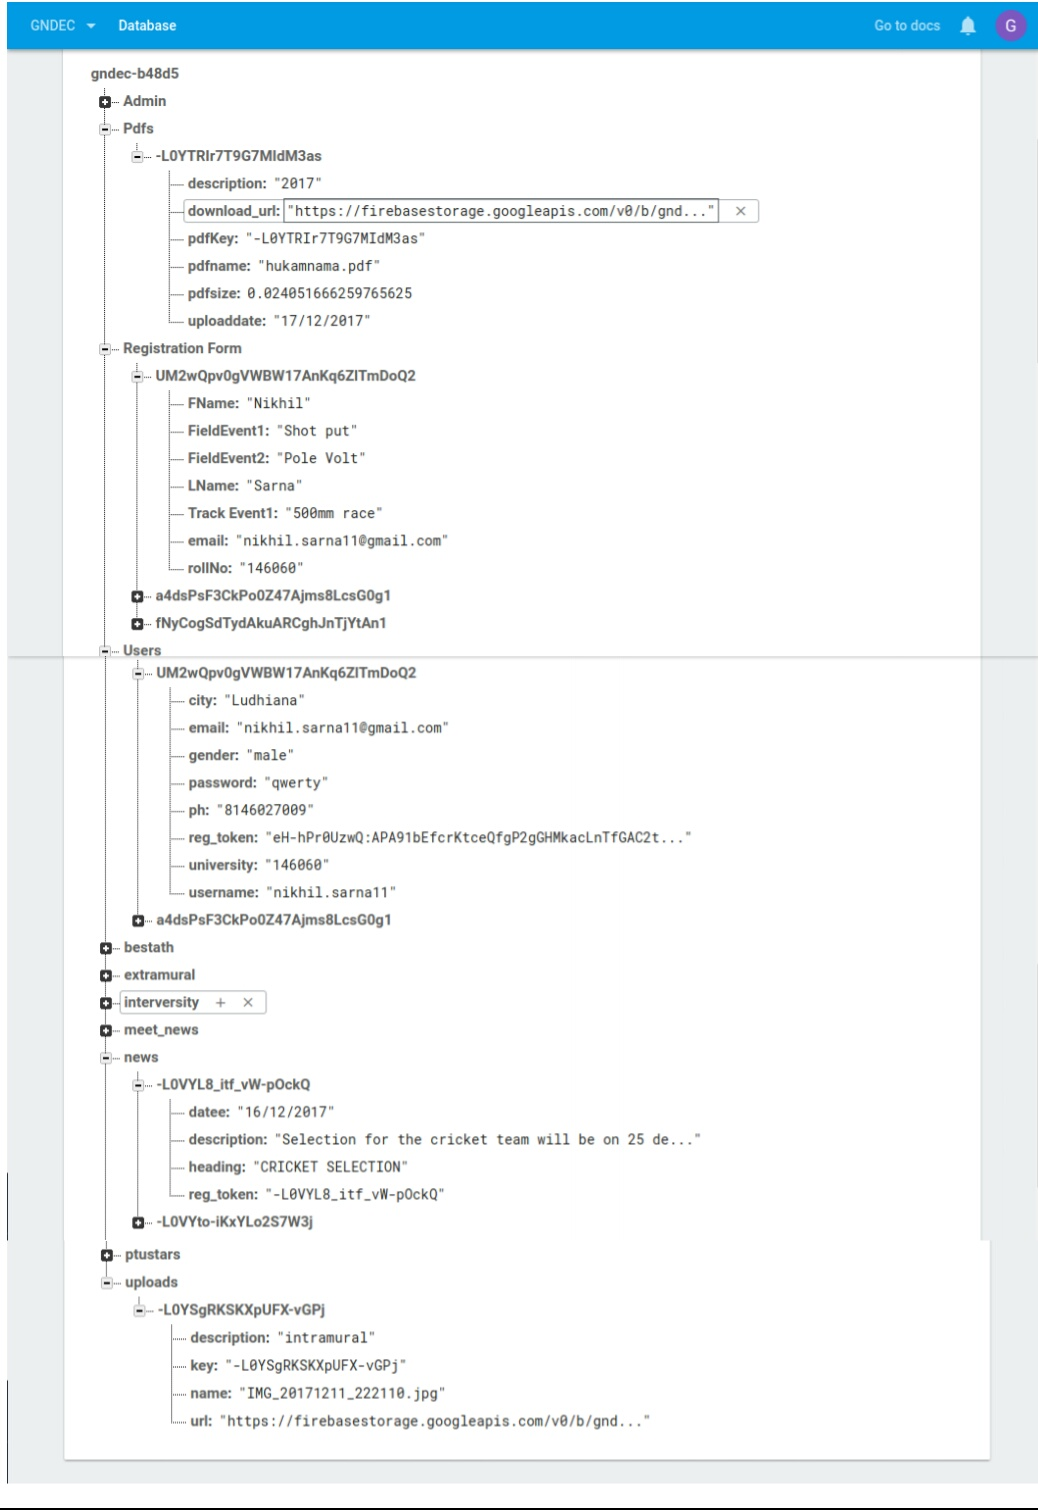
\includegraphics[scale=0.30]{images/dbfire.jpg}
		\caption{Database}
	\end{figure}






\chapter{Conclusion and Future Scope}
\section{Conclusion}
With the coming of the retinal image enhancement, there will be an easy for the doctors to detect disease from the enhanced retinal image of the patient . 

\section{Future Scope}
This application have very high future scope. With the launch of retinal image enhacement, medical staff will get benifits such as early detection of diseases from enhaced retina image. Our project can be installed in hospitals where eyes specialist can use the product made by our team.	   
\begin{thebibliography}{3}
\bibitem{} DRIVE: Digital Retinal Images for Vessel Extraction ~https://www.isi.uu.nl/Research/Databases/DRIVE/
\bibitem{} https://in.mathworks.com/
\bibitem{} https://docs.opencv.org/2.4/doc/tutorials/tutorials.html https://firebase.google.com/docs/android/setup/
\end{thebibliography}
\end{document}